\documentclass[11pt,a4paper]{article}

\usepackage[utf8]{inputenc}
\usepackage[T1]{fontenc}
\usepackage[margin=1in]{geometry}
\usepackage{setspace}
\setstretch{1.15}

\usepackage{amsmath,amssymb,amsfonts}
\usepackage{graphicx}
\usepackage{booktabs,multirow}
\usepackage{xcolor,colortbl}
\usepackage{tikz}
\usetikzlibrary{positioning,calc,arrows.meta}
\usepackage{caption}
\usepackage[edges]{forest}
\usepackage{float}
\usepackage{microtype}

% Tighten line-breaking tolerance so that long technical compounds
% (e.g. "$\mu$-parameterized", "privacy-preserving") do not overflow the margin.
\tolerance=3000
\emergencystretch=3em
\hbadness=10000
\vbadness=10000
\usepackage[normalem]{ulem}


% ---------------------------------------------------------------------------
% Revision markup, per the editor's instruction to show changes "in red font".
%
% Two grammatical forms are needed and they use DIFFERENT devices:
%   * inline  \revadd / \revdel        -- argument-delimited, one phrase long
%   * block   \revaddblock / \revdelblock -- may span several paragraphs and may
%     contain \item, \subsection, & or a display environment
%
% ulem's \uwave / \sout cannot cross a paragraph break or an environment
% boundary ("Paragraph ended before \@textcolor was complete"), so the block
% form scopes a colour group and delegates the decoration to \markadd / \markdel,
% which are applied to each surviving paragraph individually.  A payload that is a
% sectioning command (\subsection{...}) is left in flat colour: ulem cannot stroke
% a heading, and the journal's own latexdiff redline cannot either.
%
% Colour code: insertions blue + wavy underline, deletions red + strikethrough.
% ---------------------------------------------------------------------------
\newcommand{\revadd}[1]{{\color{blue}\uwave{#1}}}
\newcommand{\revdel}[1]{{\color{red}\sout{#1}}}
\newcommand{\revadddec}[1]{{\color{blue}\uwave{#1}}}
\newcommand{\revdeldec}[1]{{\color{red}\sout{#1}}}
\newcommand{\revaddblock}[1]{{\color{blue}#1}}
\newcommand{\revdelblock}[1]{{\color{red}#1}}
% Paragraph-level decoration used inside the block markers above.  The clean
% master defines \markdel as a no-op and \markadd as the identity, so both
% masters still typeset exactly the same characters.
\newcommand{\markadd}[1]{{\color{blue}\uwave{#1}}}
\newcommand{\markdel}[1]{{\color{red}\sout{#1}}}
% ulem cannot set a multi-key \citep{a,b} inside \uwave / \sout (it raises
% "Extra }, or forgotten \endgroup").  Boxing the citation first makes it an
% ordinary hbox, which ulem handles fine.  The clean master defines this macro
% as a no-op, so the two PDFs stay textually identical.
\newcommand{\citebox}[1]{\mbox{#1}}
% Invisible in the clean manuscript; in the marked-up version it flags each secondary
% subheading that was removed, so the editor can verify the restructuring point by point.
\newcommand{\revnote}[1]{\textcolor{red}{\footnotesize[#1]}}


\usepackage[numbers,sort&compress]{natbib}
\usepackage[colorlinks=true,linkcolor=blue!70!black,citecolor=blue!70!black,urlcolor=blue!70!black]{hyperref}

% npj Artificial Intelligence requirement: unnumbered section headings
\setcounter{secnumdepth}{0}

% Title, Authors, and Affiliations
\title{\Large\textbf{Financial Time-Series Generation: A Systematic Survey of Taxonomy, Evaluation, Datasets, and Open Challenges}\\[0.4em]\normalsize\textbf{[Marked-up manuscript: insertions in blue, deletions struck through in red]}}

\author{
  Yingxiao Zhang$^{1,2}$, 
  Jiaxin Duan$^{3}$, 
  Yue Zou$^{1,2}$, 
  Ke Feng$^{1,*}$, 
  Jing Xiao$^{4,*}$
}

\date{}

\begin{document}

\maketitle

\vspace{-2em}
\begin{center}
\footnotesize
$^{1}$School of Software and Microelectronics, Peking University, Beijing, China\\[0.3em]
$^{2}$Pingan Bank Co., Ltd., Shenzhen, China\\[0.3em]
$^{3}$China Electronics Cloud Technology Co., Ltd., Beijing, China\\[0.3em]
$^{4}$Pingan Group Co., Ltd., Shenzhen, China\\[0.5em]
$^{*}$Corresponding authors. E-mail: \texttt{fengke@pku.edu.cn} (K. Feng); \texttt{xiaojing661@pingan.com.cn} (J. Xiao)
\end{center}
\vspace{1.5em}

% Abstract (single paragraph, 150-200 words, no subheadings)
\begin{abstract}
The rapid advancement of generative artificial intelligence has catalyzed a paradigm shift in quantitative finance, transitioning from traditional point forecasting toward comprehensive financial time-series generation (FTSG) across extrapolation, imputation, and full-scale data synthesis. This transition is motivated by the critical need to simulate rare market regimes, reconstruct incomplete historical records, and produce privacy-preserving synthetic environments for stress testing and trading execution. However, empirical financial properties---including heavy tails, volatility clustering, non-stationarity, and regime shifts---pose severe hurdles for generic generative frameworks. In this systematic survey, we review \revdeldec{ 130 }\revadddec{131 }studies from 2021 to early 2026 to bridge the gap between machine learning capabilities and econometric validity. We introduce a two-level taxonomy structuring the domain across task formulations and algorithmic families, and establish a multi-dimensional evaluation protocol encompassing distributional fidelity, stylized facts preservation, and downstream utility. Furthermore, we catalog curated financial databases and benchmark suites while addressing empirical dataset construction pitfalls. Finally, we identify pivotal open challenges in causal representation learning, econometrically bounded modeling, and online adaptation under distribution shifts. This review provides a standardized roadmap for developing robust, domain-aligned financial generative models.
\end{abstract}

% Introduction (no subheadings)
\section{Introduction}
\label{sec:1}

Time-series analysis (TSA)~\revaddblock{\citep{hamilton1994time,box2015time} }has long been a central pillar of quantitative finance\revaddblock{~\citep{campbell1997econometrics,tsay2010analysis}}, providing the mathematical foundation for modeling market dynamics, assessing risk, and pricing \revdelblock{ complex assets~
}\revaddblock{assets}. Traditionally, TSA in finance was \revdelblock{ synonymous with forecasting}\revaddblock{closely associated with forecasting~\citep{hyndman2021forecasting}}: predicting the next price movement, the future volatility level, or the impending macroeconomic shift. \revdelblock{ However, as }\revaddblock{Modern probabilistic forecasting goes beyond point estimates by quantifying predictive distributions and forecast uncertainty~\citep{gneiting2014probabilistic}. As }the financial industry becomes increasingly data-driven and algorithmic, the demand has evolved from \revdelblock{ mere }point estimation to the comprehensive generation of plausible market scenarios. This paradigm shift has given rise to Financial Time-Series Generation (FTSG), \revdelblock{ a domain that extends beyond }\revaddblock{which extends conventional }forecasting to include \revdelblock{ the synthesis of entirely new data, the imputationof incomplete price records, and the extrapolation of diverse financial products}\revaddblock{fully synthetic financial sequences~\citep{Time-GAN,wiese2020,naritomi2020data}, missing-data imputation~\citep{yoon2018gain,tashiro2021csdi,wang2024cwgain}, and probabilistic extrapolation of future financial trajectories~\citep{rasul2021timegrad}}.

The motivation for FTSG is deeply rooted in the structural limitations of real-world financial data. Unlike text or images, financial markets are characterized by a low signal-to-noise ratio, extreme non-stationarity, and abrupt regime shifts triggered by geopolitical events or macroeconomic policy changes. Furthermore, empirical financial distributions frequently exhibit "stylized facts" such as heavy tails, volatility clustering, and leverage effects\revaddblock{~\citep{cont2001empirical}}. While historical data contains instances of these phenomena, critical events like market crashes or sudden liquidity droughts are inherently rare. Consequently, discriminative models trained solely on historical records often suffer from overfitting and fail to generalize during crises. FTSG \revdelblock{ addresses }\revaddblock{can address }this by creating high-fidelity\revdelblock{ , }\revaddblock{—and, when trained with formal privacy controls, potentially }privacy-preserving\revaddblock{—}synthetic data that can augment training sets, simulate counterfactual stress-testing scenarios, and train robust reinforcement learning agents in simulated environments.

Across the task taxonomy of this survey, we use \revdelblock{ \textbf{FTSG} }\revaddblock{FTSG }to denote the umbrella research domain (Financial Time-Series Generation), while \revdelblock{ \textbf{FTSE}, \textbf{FTSI}, and \textbf{FTSS} }\revaddblock{FTSE, FTSI, and FTSS }denote the three task-level formulations for extrapolation, imputation, and synthesis, respectively. This terminology is used consistently throughout the paper and is summarized again in the Problem Formulation and Taxonomy and Applications sections.

\revdelblock{ The rapid integration of Generative AI (GAI), as demonstrated }\revaddblock{Generative AI has rapidly entered financial modeling, as illustrated }in Figure~\ref{fig:timeline}\revdelblock{ , including Generative Adversarial Networks }\revaddblock{. The main families include generative adversarial networks }(GANs)\revdelblock{ 
, Denoising Diffusion Probabilistic Models }\revaddblock{~\citep{goodfellow2014gan,Time-GAN,wiese2020,naritomi2020data}, denoising diffusion probabilistic models }(DDPMs)~\citep{ho2020ddpm,rasul2021timegrad}, \revdelblock{ and Large Language Models }\revaddblock{Transformers~\citep{vaswani2017attention} and large language models }(LLMs)\revdelblock{ 
---into financial modeling has }\revaddblock{~\citep{brown2020language,jin2024timellm,ansari2024chronos}. These developments, together with their financial adaptations, have }produced a fragmented and rapidly expanding body of literature. \revdelblock{ While several surveys have attempted to capture these advancements 
, they suffer from notable limitations in technical and methodological aspects}\revaddblock{Zhang et al.~\citep{Survey1} survey LLMs for time series, while Liang et al.~\citep{Survey2} review time-series foundation models. Kim et al.~\citep{Survey3} and Kong et al.~\citep{Survey4} review deep time-series forecasting architectures, and Nie et al.~\citep{FinSurvey1} and Arsenault et al.~\citep{FinSurvey3} review financial-AI applications. These surveys help map parts of the literature, but they leave several task- and evaluation-oriented gaps}.

First, the majority of existing surveys remain heavily skewed toward forecasting (extrapolation) and classification, often treating generation merely as an auxiliary data augmentation step rather than a standalone class of problems encompassing synthesis and imputation. Second, \revdelblock{ most reviews are organized strictly by model architecture (e.g., "A Survey of LLMs in Finance" or "Diffusion Models for Time Series"), which obscures the fundamental }\revaddblock{the reviews by Zhang et al.~\citep{Survey1} and Liang et al.~\citep{Survey2} are organized primarily around model families and representation-learning components, whereas the reviews by Kim et al.~\citep{Survey3}, Kong et al.~\citep{Survey4}, Nie et al.~\citep{FinSurvey1}, and Arsenault et al.~\citep{FinSurvey3} emphasize architectures or application domains; this organization obscures }differences in task formulation, supervision signals, and conditioning contexts\revdelblock{ inherent in financial applications}. Third, and most critically, existing literature lacks a systematic discussion on evaluation protocols. Assessing a synthetic financial sequence requires moving beyond generic point-wise error metrics (like MSE or MAE) to evaluate cross-sectional dependence, tail-risk preservation, and downstream utility---areas where current surveys offer little standardization or critical synthesis. Finally, there is a scarcity of resource-oriented reviews that comprehensively catalog financial benchmarks, datasets, and the practical biases (e.g., survivorship bias) that plague empirical financial research.

To substantiate these gaps concretely, Table~\ref{tab:related_surveys} positions our survey against the six prior surveys cited above along five explicit dimensions: task coverage (whether each of the three FTSG sub-tasks---extrapolation (FTSE), imputation (FTSI), and synthesis (FTSS)---is treated as a first-class topic), evaluation treatment (whether a multi-dimensional protocol is provided, beyond per-paper metric tables), dataset cataloging (whether FTSG-relevant financial benchmarks are systematically inventoried), number of references in the bibliography \revaddblock{(coded approximately from the available versions)}, and time window of coverage. \revdelblock{ The table confirms }\revaddblock{Our coding suggests }that no prior survey jointly covers all three FTSG sub-tasks with a dedicated evaluation protocol and a curated financial dataset catalog; each gap maps to one of the four motivating critiques above and motivates a corresponding contribution of our survey discussed below.

To address these critical gaps, this paper provides a systematic, evaluation-oriented survey of FTSG, focusing on the intersection of generative AI and financial econometrics over the past five years (2021--early 2026). We elevate the discourse from a mere enumeration of literature to a structured problem formulation and benchmarking perspective. Our \revdelblock{ main }contributions are fourfold\revdelblock{ :




\textbf{A Task-Technique Two-Level Taxonomy}: }\revaddblock{. First, we propose a task-technique two-level taxonomy. }By comprehensively reviewing \revdelblock{ 130 }\revaddblock{131 }studies published in 2021--early 2026, we \revdelblock{ propose a novel }\revaddblock{develop a }hierarchical classification system that decouples the \textit{what} (extrapolation, imputation, \revaddblock{and }synthesis) from the \textit{how} (statistical, deep discriminative, GAN\revdelblock{ s}, diffusion, \revdelblock{ foundation models}\revaddblock{and foundation-model approaches}), enabling a clearer mapping of \revdelblock{ specific }generative techniques to \revdelblock{ their optimal }financial use cases. \revdelblock{ 
\textbf{A Systematic Evaluation Framework}: We introduce a comprehensive, multi-dimensional evaluation protocol for FTSG . Moving }\revaddblock{Second, we establish a systematic evaluation framework for FTSG that moves }beyond generic reconstruction metrics \revdelblock{ , we establish a unified checklist encompassing }\revaddblock{to encompass }distributional fidelity, \revdelblock{ stylized facts }\revaddblock{stylized-facts }preservation, downstream utility, and robustness \revdelblock{ against }\revaddblock{to }regime shifts. \revdelblock{ 
\textbf{A Comprehensive Resource Synthesis}: We }\revaddblock{Third, we }compile and categorize \revdelblock{ a wide array of }public data resources, APIs, and emerging benchmark suites\revdelblock{ (e.g., }\revaddblock{, including }FinTSB \citep{hu2025fintsb} \revdelblock{ , }\revaddblock{and }TFB \citep{TFB}\revdelblock{ ) }\revaddblock{, }specifically relevant to financial generation, \revdelblock{ alongside a critical discussion of practical dataset construction issues. 
\textbf{Identification of Open Challenges}: We synthesize the literature to identify critical bottlenecks }\revaddblock{and discuss practical issues in dataset construction. Fourth, we synthesize open challenges }in financial validity \revdelblock{ , proposing }\revaddblock{and identify }actionable future directions\revdelblock{ such as }\revaddblock{, including }financial-theory-informed generative modeling and causal representation learning.

% 【文生图】 [A flow diagram illustrating the mapping from financial generation tasks (extrapolation, imputation, synthesis) to practical downstream applications (risk warning, data repair, stress testing, simulation). Style: Professional academic flowchart, Information Sciences journal aesthetic, clear directional arrows.]




The remainder of this paper is organized according to the IRDM structure. The Results section presents our core survey findings across six thematic \revdelblock{ subsections}\revaddblock{areas}: problem formulation and two-level taxonomy, task-specific analyses of extrapolation, imputation, and synthesis, downstream quantitative applications, evaluation protocols for financial realism, and data resources with benchmarks. The Discussion section critically examines pressing open challenges and future research directions, synthesizing the implications for financial generative modeling. Finally, the Methods section details the systematic literature retrieval strategy \revdelblock{ , }\revaddblock{and }PRISMA-compliant screening protocol\revaddblock{~\citep{page2021prisma}}, inclusion criteria, and coding procedures governing this survey.

% Results (compulsory subheadings)
\section{Results}
\subsection{Problem Formulation and \revdelblock{ A Two-Level Taxonomy}\revaddblock{Setup}}
\label{sec:taxonomy}

% \definecolor{ColorExtrapolation}{RGB}{240, 245, 255}
% \definecolor{ColorImputation}{RGB}{240, 255, 240}
% \definecolor{ColorAugmentation}{RGB}{255, 245, 235}
% \definecolor{BorderGray}{RGB}{180, 180, 180}

\definecolor{ColorExtrapolation}{RGB}{240, 245, 255}
\definecolor{ColorImputation}{RGB}{240, 255, 240}
\definecolor{ColorAugmentation}{RGB}{255, 245, 235}
\definecolor{BorderGray}{RGB}{180, 180, 180}

\revdelblock{ \subsection{Problem Setup}
}To establish a rigorous conceptual foundation, Figure~\ref{fig:taxonomy} presents a comprehensive two-level hierarchical taxonomy that structures the entire financial time-series generation landscape across task formulations and algorithmic families.
Let $\mathbf{X} = \{x_1, x_2, \dots, x_T\}$ denote a multivariate financial time series, where each $x_t \in \mathbb{R}^d$ represents a vector of financial variables (e.g., asset prices, returns, trading volumes, or limit order book states) at time step $t$. Financial time series are inherently stochastic, heavily influenced by non-stationary market regimes, and exhibit complex inter-variable dependencies.
The core objective of Financial Time-Series Generation (FTSG) is to learn a probabilistic generative model $P_\theta$ capable of producing synthetic sequences $\hat{\mathbf{X}}$ that capture both the marginal distributions and the temporal dynamics of the true data-generating process $P_{data}$.

\subsection{Task-Level Taxonomy}
As illustrated in Figure~\ref{fig:tasks}, \revdelblock{ we organize FTSG into }\revaddblock{FTSG comprises }three distinct problem formulations based on \revdelblock{ the generation context:


\textbf{Financial Time-Series Extrapolation:} A }\revaddblock{generation context.

Financial time-series extrapolation is a }conditional, forward-looking generation task. Given a historical prefix $\mathbf{x}_{1:t}$, the goal is to generate future trajectories $\mathbf{x}_{t+1:T}$. The predictive distribution is modeled as $P(\mathbf{x}_{t+1:T} \mid \mathbf{x}_{1:t}; \theta) = \prod_{i=t+1}^{T} P(x_i \mid \mathbf{x}_{1:i-1}; \theta)$. This encompasses probabilistic forecasting, where the output is a set of plausible future paths rather than a single point estimate.

\revdelblock{ 
\textbf{Financial Time-Series Imputation:} A }\revaddblock{Financial time-series imputation is a }bidirectional, closed-format generation task. Let $\mathbf{M} \in \{0, 1\}^T$ be a binary mask indicating missing values. Given an incomplete sequence with missing elements $\mathbf{x}_{miss} = \mathbf{x} \odot \mathbf{M}$ and observed elements $\mathbf{x}_{obs} = \mathbf{x} \odot (1-\mathbf{M})$, the objective is to reconstruct the missing data while preserving local and global statistical coherence: $P(\mathbf{x}_{miss} \mid \mathbf{x}_{obs}; \theta)$.

\revdelblock{ 
\textbf{Synthetic Sequence Generation / Data Synthesis:} An unconditional or conditionally-guided }\revaddblock{Synthetic sequence generation, or data synthesis, is an unconditional or conditionally guided }generation task aimed at creating entirely new data manifolds. The model learns to map a latent noise variable $\mathbf{z} \sim \mathcal{N}(0, \mathbf{I})$ (and optionally a condition $c$ such as market regime or volatility target) to a realistic sequence: $\hat{\mathbf{X}} = G_{\theta}(\mathbf{z}, c)$, aiming to minimize the divergence between the generated distribution $P_g$ and the real distribution $P_{data}$.

\subsection{Technique-Level Taxonomy}
To map the rapid evolution of algorithmic approaches, \revdelblock{ we classify }the underlying generative techniques \revdelblock{ into the following families:


\textbf{Statistical and Probabilistic Methods:} Classical }\revaddblock{can be grouped into six families.

Statistical and probabilistic methods include classical }approaches such as ARIMA\revdelblock{ and GARCH}\revaddblock{~\citep{box1970} and GARCH~\citep{bollerslev1986garch}}, which model conditional mean and variance based on rigid mathematical assumptions.

\revdelblock{ 
\textbf{Discriminative Deep Sequence Models:} Recurrent Neural Networks }\revaddblock{Discriminative deep sequence models include recurrent neural networks }(RNNs)\revdelblock{ and hybrid LSTMs }\revaddblock{~\citep{elman1990finding} and long short-term memory (LSTM) networks~\citep{hochreiter1997lstm} }optimized via pointwise loss functions.

\revdelblock{ 
\textbf{Adversarial Generative Models (GANs):} Frameworks utilizing }\revaddblock{Adversarial generative models (GANs)~\citep{goodfellow2014gan} use }generator-discriminator dynamics\revdelblock{ (e.g., }\revaddblock{, including the Wasserstein GAN with gradient penalty (}WGAN-GP)\revaddblock{~\citep{arjovsky2017wgan,gulrajani2017wgangp}, }to implicitly learn the data distribution.

\revdelblock{ 
\textbf{Diffusion / Score-Based Models:} Models that }\revaddblock{Diffusion and score-based models~\citep{ho2020ddpm,song2019generative,song2021score} }learn to reverse a gradual noising process, offering stable training and high-fidelity distribution matching.

\revdelblock{ 
\textbf{Foundation Models / LLM-Based Models:} Recent }\revaddblock{Foundation models and LLM-based models are recent }adaptations of large pre-trained \revdelblock{ transformers }\revaddblock{Transformers~\citep{vaswani2017attention,brown2020language} }to the time-series domain, \revdelblock{ enabling zero-shot generation and cross-modal reasoning.

\textbf{Controllable and Multimodal Generative Models:} Advanced architectures }\revaddblock{represented by models such as Chronos~\citep{ansari2024chronos}, OneFitsAll~\citep{zhou2023onefitsall}, and Time-LLM~\citep{jin2024timellm}.

Controllable and multimodal generative models, including TimeWeaver~\citep{narasimhan2024timeweaver}, T2S~\citep{T2S}, and dual-sourced text--time diffusion models~\citep{lozano2023dual}, are }designed to generate sequences conditioned on textual instructions, macroeconomic indicators, or specific volatility regimes.

The detailed classification of FTSG methods, organized by task and technique, is summarized in Figure ~\ref{fig:taxonomy} for a clear overview.

\subsection{Mapping Tasks to Techniques}
Table \ref{tab:mapping} provides a unified mapping of these tasks to the corresponding techniques, highlighting the evolution from deterministic prediction to flexible, scenario-based generative paradigms. Specifically, for the extrapolation task, the landscape spans from deep sequence architectures \revdelblock{ (e.g., }\revaddblock{such as }SGP-LSTM\revdelblock{ ) }\revaddblock{~\citep{SGP-LSTM1} }that forecast prices and returns using deterministic metrics like MSE, to advanced diffusion and foundation models \revdelblock{ (e.g., TimeGrad}\revaddblock{such as TimeGrad~\citep{rasul2021timegrad}, Chronos~\citep{ansari2024chronos}}, \revdelblock{ Chronos, }and FinCast\revdelblock{ )}\revaddblock{~\citep{zhu2025fincast}}. These newer paradigms handle multivariate and multi-asset series, shifting the evaluation focus toward \revdelblock{ probabilistic measures }\revaddblock{proper probabilistic scoring rules such as the continuous ranked probability score }(CRPS)\revaddblock{~\citep{gneiting2007strictly} }and zero-shot capabilities. In the realm of imputation, missing fundamentals and prices are primarily addressed using tensor methods \revdelblock{ (RegTensor) }\revaddblock{such as RegTensor~\citep{zhou2023regtensor} }and diffusion models \revdelblock{ (CSDI, TimeDiT)}\revaddblock{such as CSDI~\citep{tashiro2021csdi} and TimeDiT~\citep{cao2024timedit}}, where performance is gauged by reconstruction error and temporal coherence. Finally, for data synthesis, generative frameworks such as QuantGAN\revdelblock{ and CoFinDiff }\revaddblock{~\citep{wiese2020} and CoFinDiff~\citep{tanaka2025cofindiff} }are employed to simulate realistic returns, market scenarios, and complex limit order flows. Consequently, the evaluation criteria for synthesis shift entirely away from point-wise accuracy, prioritizing instead the preservation of stylized facts, distributional fidelity, and the practical downstream utility of the generated data.


\subsection{Financial Time-Series Extrapolation}
\label{sec:extrapolation}

\subsubsection{Problem Characteristics}
Financial Time-Series Extrapolation (FTSE) is formally defined as the task of generating future trajectories $\mathbf{x}_{t+1:T}$ given a historical context $\mathbf{x}_{1:t}$. Unlike traditional point forecasting, modern FTSE is approached as a probabilistic conditional generation problem: learning the conditional distribution $p(\mathbf{x}_{t+1:T} | \mathbf{x}_{1:t})$ to capture the inherent uncertainty and multi-modal nature of financial markets. This shift acknowledges that financial markets are stochastic systems with complex, time-varying dynamics. 

The problem exhibits several distinct characteristics that differentiate it from general sequence extrapolation:
\begin{enumerate}
    \item \textbf{Causality Constraint}: The generation must be strictly causal—future values depend solely on past observations without any look-ahead bias. This is analogous to autoregressive language modeling, but with continuous, real-valued tokens.
    \item \textbf{Non-Stationarity}: Financial time series exhibit time-varying statistical properties (e.g., changing volatility regimes, structural breaks). The conditional distribution $p(\mathbf{x}_{t+1:T} | \mathbf{x}_{1:t})$ itself evolves over time, requiring models to adapt to distributional shifts.
    \item \textbf{Low Signal-to-Noise Ratio}: Market data is dominated by noise, making it challenging to separate genuine predictive signals from random fluctuations. This often leads to overfitting in deterministic models.
    \item \textbf{High-Dimensional Dependencies}: In multi-variate settings, assets exhibit complex cross-sectional dependencies (e.g., lead-lag relationships, sector correlations). Modeling these dependencies is crucial for coherent joint generation.
\end{enumerate}

Formally, the objective is to learn a generator $G_\theta$ that maps the context $\mathbf{x}_{1:t}$ to a distribution over future sequences, often parameterized as a set of samples $\{\mathbf{x}_{t+1:T}^{(i)}\}_{i=1}^N$. The evaluation metrics extend beyond point-wise accuracy (e.g., MSE) to probabilistic scoring rules (e.g., CRPS, Energy Score) and domain-specific financial utility measures (e.g., portfolio returns, risk metrics).


\subsubsection{Classical and Hybrid Predictive Models}

Classical statistical frameworks have historically provided the mathematical bedrock for modeling financial time-series dynamics through rigorous probabilistic assumptions. A prominent example is the Auto-Regressive Integrated Moving Average (ARIMA) model \citep{box1970}, which explicitly formulates temporal dependencies by combining autoregressive (AR) processes, differencing (I) to achieve stationarity, and moving average (MA) components. For a given time series $y_t$, an $\text{ARIMA}(p, d, q)$ specification is mathematically expressed as:
\begin{equation}
\nabla^d y_t = c + \sum_{i=1}^p \phi_i \nabla^d y_{t-i} + \sum_{j=1}^q \theta_j \varepsilon_{t-j} + \varepsilon_t
\end{equation}
where $\nabla^d$ represents the $d$-th order difference operator, $\phi_i$ and $\theta_j$ are the AR and MA coefficients respectively, and $\varepsilon_t \sim \mathcal{N}(0, \sigma^2)$ acts as white noise. While ARIMA models are effective at isolating linear relationships, they inherently fail to encompass complex market phenomena such as volatility clustering and heavy-tailed distributions. To capture these time-varying variance dynamics, the Generalized Autoregressive Conditional Heteroskedasticity (GARCH) framework \citep{kim2021} was introduced. The conditional variance $\sigma_t^2$ in a $\text{GARCH}(p, q)$ model is iteratively defined by past squared innovations and past variances:
\begin{equation}
\sigma_t^2 = \omega + \sum_{i=1}^p \alpha_i \varepsilon_{t-i}^2 + \sum_{j=1}^q \beta_j \sigma_{t-j}^2
\end{equation}
where $\omega > 0$, $\alpha_i \ge 0$, and $\beta_j \ge 0$. Although extensions like EGARCH further accommodate asymmetric leverage effects resulting from negative shocks, these purely parametric methods struggle to scale to high-dimensional dependencies and intricate non-linear patterns.

To address the constraints of classical statistical models, the field transitioned toward deep learning architectures, particularly Recurrent Neural Networks (RNNs) and Long Short-Term Memory (LSTM) networks \citep{tsa1, qin2025, li2025ceemdan, caliskan2025, SGP-LSTM1}. LSTMs leverage a sophisticated gating mechanism—comprising forget ($f_t$), input ($i_t$), and output ($o_t$) gates alongside a cell state ($C_t$) and hidden state ($h_t$)—to effectively capture long-range temporal dependencies without suffering from severe vanishing gradients:
\begin{align}
f_t &= \sigma(\mathbf{W}_f \cdot[h_{t-1}, x_t] + b_f) \\
i_t &= \sigma(\mathbf{W}_i \cdot [h_{t-1}, x_t] + b_i) \\
\tilde{C}_t &= \tanh(\mathbf{W}_C \cdot[h_{t-1}, x_t] + b_C) \\
C_t &= f_t \odot C_{t-1} + i_t \odot \tilde{C}_t \\
o_t &= \sigma(\mathbf{W}_o \cdot [h_{t-1}, x_t] + b_o) \\
h_t &= o_t \odot \tanh(C_t)
\end{align}
However, when standard LSTMs are optimized using traditional pointwise loss functions such as the Mean Squared Error (MSE), defined as $\mathcal{L}_{MSE} = \frac{1}{n} \sum_{i=1}^n (y_i - \hat{y}_i)^2$, they often overfit the ubiquitous noise present in financial data.

Consequently, recent literature has pivoted towards sophisticated hybrid strategies that couple deep learning backbones with domain-specific signal processing or invariant learning techniques to enhance robustness. Denoising-based hybrids, for example, incorporate explicit signal decomposition to systematically separate underlying predictive trends from stochastic market noise. The PEC-W model \citep{caliskan2025} leverages the Discrete Wavelet Transform (DWT) to split raw input series into multi-resolution scale and wavelet representations:
\begin{equation}
x(t) = \sum_k c_{J,k} \phi_{J,k}(t) + \sum_{j=1}^J \sum_k d_{j,k} \psi_{j,k}(t)
\end{equation}
where $\phi$ and $\psi$ denote the scaling and wavelet functions. These denoised approximation coefficients provide a cleaner input signal for the LSTM, a concept similarly explored by CEEMDAN (Complete Ensemble Empirical Mode Decomposition with Adaptive Noise)-Informer-LSTM \citep{li2025ceemdan}, which decomposes the signal into intrinsic mode functions. Beyond denoising, feature engineering hybrids seek to automate the discovery of robust predictive inputs. The SGP-LSTM framework \citep{SGP-LSTM1} employs Symbolic Genetic Programming to iteratively evolve technical indicators, steering the search via a multi-objective fitness function that balances return, consistency, and predictive correlation (IC):
\begin{equation}
\text{Fitness} = \text{TopR} + \lambda_1 \times \text{Monotonicity} + \lambda_2 \times \text{IC}
\end{equation}
Finally, invariant learning hybrids target the problem of distributional shifts across varying market regimes. The Invariant Risk Minimization (IRM) approach proposed by \citet{cao2023irm} enforces the extraction of representations that hold true regardless of whether the market is in a bullish, bearish, or sideways phase, minimizing an objective that penalizes environmental variance:
\begin{equation}
\mathcal{L}_{IRM} = \underbrace{R^e(\mathbf{w} \cdot \Phi)}_{\text{Empirical risk}} + \gamma \underbrace{\left\| \nabla_{\mathbf{w}|_{\mathbf{w}=1.0}} R^e(\mathbf{w} \cdot \Phi) \right\|_2^2}_{\text{Invariant penalty}}
\end{equation}
where $\Phi$ acts as the representation function and $\mathbf{w}$ is a linear classifier. Despite these multifaceted improvements, hybrid predictive architectures ultimately generate deterministic point forecasts, fundamentally limiting their capacity to model the full predictive distribution essential for robust financial scenario generation.

\subsubsection{Generative Models for Extrapolation}

Recognizing the intrinsic limitations of deterministic forecasting, the paradigm of generative models shifts the focus toward learning the underlying data distribution $p(\mathbf{x})$ or the conditional probability $p(\mathbf{x}_{t+1:T}|\mathbf{x}_{1:t})$. This transition allows practitioners to sample multiple plausible future trajectories, accommodating the multi-modal uncertainty inherent in financial markets. Early efforts in this domain heavily utilized Generative Adversarial Networks (GANs) \citep{Time-GAN, naritomi2020data}, which deploy a generator $G$ and a discriminator $D$ locked in a competitive minimax game. The generator synthesizes sequences from historical context $\mathbf{x}_{1:t}$ and a latent noise vector $\mathbf{z}$, while the discriminator attempts to distinguish real historical samples from the generated distributions:
\begin{equation}
\min_G \max_D \mathbb{E}_{\mathbf{x} \sim p_{data}}[\log D(\mathbf{x})] + \mathbb{E}_{\mathbf{z} \sim p_z}[\log(1 - D(G(\mathbf{z})))]
\end{equation}
While conceptually elegant, GANs are notoriously difficult to train on volatile financial data, frequently suffering from mode collapse and unstable convergence. To mitigate these issues, specialized adaptations have been devised. WaveGAN \citep{dai2024wavegan} incorporates a multi-resolution DWT denoising mechanism combined with a Wasserstein GAN equipped with Gradient Penalty (WGAN-GP) \citep{wang2024denoiser}. The WGAN-GP loss enforces a Lipschitz constraint to prevent vanishing gradients:
\begin{equation}
\mathcal{L}_{\text{WGAN-GP}} = \mathbb{E}_{\tilde{\mathbf{x}} \sim p_g}[D(\tilde{\mathbf{x}})] - \mathbb{E}_{\mathbf{x} \sim p_{data}}[D(\mathbf{x})] + \lambda \mathbb{E}_{\hat{\mathbf{x}} \sim p_{\hat{\mathbf{x}}}}[(\|\nabla_{\hat{\mathbf{x}}} D(\hat{\mathbf{x}})\|_2 - 1)^2]
\end{equation}
where $\hat{\mathbf{x}}$ represents a convex interpolation of real and generated instances. Concurrently, models like N-BEATS-GAN \citep{dai2026nbeats} fuse interpretable basis expansions \citep{oreshkin2020nbeats} with an adversarial framework, modeling future values as a sum of trend and seasonality bases $\hat{\mathbf{y}} = \sum_{i=1}^N \text{Basis}_i(\boldsymbol{\theta}_i)$. While these modifications enhance stability and interpretability, GANs often yield over-smoothed samples that fail to encapsulate the sharp, multi-modal nature of empirical return distributions.

To achieve higher fidelity in distribution matching, Denoising Diffusion Probabilistic Models (DDPMs) \citep{ho2020ddpm} have emerged as a more stable and expressive alternative. Diffusion frameworks systematically destroy structured data by injecting Gaussian noise over $T$ forward steps—$q(\mathbf{x}_t|\mathbf{x}_{t-1}) = \mathcal{N}(\mathbf{x}_t; \sqrt{1 - \beta_t}\mathbf{x}_{t-1}, \beta_t \mathbf{I})$—and then learn a parameterized reverse process $p_\theta(\mathbf{x}_{t-1}|\mathbf{x}_t) = \mathcal{N}(\mathbf{x}_{t-1}; \boldsymbol{\mu}_\theta(\mathbf{x}_t, t), \sigma_t^2 \mathbf{I})$ to reconstruct the signal. The optimization simplifies to predicting the incrementally added noise $\boldsymbol{\epsilon}$:
\begin{equation}
\mathcal{L}_{simple} = \mathbb{E}_{t, \mathbf{x}_0, \boldsymbol{\epsilon}}[\|\boldsymbol{\epsilon} - \boldsymbol{\epsilon}_\theta(\mathbf{x}_t, t)\|^2]
\end{equation}
For context-conditioned financial generation, TimeGrad \citep{rasul2021timegrad} integrates an RNN-based encoder with a score-based diffusion decoder, generating future states via Langevin dynamics where the context encoding $\mathbf{c}$ steers the reverse sampling:
\begin{equation}
\mathbf{x}_{t-1} = \frac{1}{\sqrt{\alpha_t}} \left( \mathbf{x}_t - \frac{\beta_t}{\sqrt{1 - \bar{\alpha}_t}} \boldsymbol{\epsilon}_\theta(\mathbf{x}_t, t, \mathbf{c}) \right) + \sigma_t \mathbf{z}
\end{equation}
Addressing the limitations of recurrent architectures in capturing extended dependencies, TimeDiT \citep{cao2024timedit} replaces the RNN with a Diffusion Transformer. Utilizing patch embeddings and multi-head attention, TimeDiT operates on a $\mu$-parameterized loss function, explicitly aligning the predicted mean of the reverse process with its theoretical target:
\begin{equation}
\mathcal{L} = \sum_{t=1}^T \mathbb{E}_{q(\mathbf{x}_t^{tar}|\mathbf{x}_0^{con})} \left[ \|\boldsymbol{\mu}(\mathbf{x}_t^{tar}, \mathbf{x}_0^{con}) - \boldsymbol{\mu}_\theta(\mathbf{x}_t^{tar}, t|\mathbf{x}_0^{con})\|^2 \right]
\end{equation}
An alternative diffusion formulation leverages continuous-time score matching, optimizing a score network to approximate the gradient of the log-density:
\begin{equation}
\mathcal{L}_{score} = \mathbb{E}_{t, \mathbf{x}_0, \boldsymbol{\epsilon}} \left[ \left\| \boldsymbol{\epsilon} - \sigma_t \nabla_{\mathbf{x}_t} \log p_\theta(\mathbf{x}_t) \right\|^2 \right]
\end{equation}
While diffusion and score-based models generate high-fidelity distributions with sharp multi-modal properties, their iterative sampling procedures introduce significant inference latency, presenting an ongoing challenge for high-frequency financial applications.



\subsubsection{Time Series Foundation Models}

Inspired by the transformative success of Large Language Models (LLMs) in natural language processing \citep{Survey1, Survey2, tsa2}, current research is heavily invested in adapting the "pre-train, then fine-tune" paradigm to financial time-series extrapolation. These Foundation Models are trained on massive, heterogeneous datasets to derive generalized temporal representations, effectively enabling zero-shot inference and cross-domain adaptation. The primary challenge in this domain is bridging the continuous numerical space of financial data with the discrete, tokenized vocabulary natively processed by transformer-based LLMs. Tokenization-based fine-tuning strategies directly address this by casting forecasting as a next-token prediction task. For instance, Chronos \citep{ansari2024chronos} scales time-series observations and maps them into a fixed dictionary of tokens using quantile binning:
\begin{equation}
\text{token}(\mathbf{x}) = \arg\min_i |x - q_i|
\end{equation}
where $q_i$ represent pre-computed quantiles. While this approach benefits from robust zero-shot generalization, the inherent discretization process sacrifices fine-grained numerical precision. Conversely, patch-based fine-tuning techniques, as exemplified by OneFitsAll \citep{zhou2023onefitsall}, bypass discretization by segmenting the time-series into sequences of sub-series patches. Each patch is projected into the high-dimensional embedding space of the LLM via a linear transformation:
\begin{equation}
\mathbf{E}_{patch} = \mathbf{W}_p \mathbf{x}_{patch} + \mathbf{b}_p
\end{equation}
These continuous patch embeddings are then prepended as visual-like tokens, fully preserving numerical fidelity while seamlessly leveraging the LLM's cross-patch attention mechanisms.

As illustrated in Figure \ref{fig:llm_comparison}, beyond conventional fine-tuning, sophisticated model editing and reprogramming approaches have emerged to align disparate modalities using lightweight adapters, averting the computational burden of full-parameter updates. StockTime \citep{wang2024stocktime} enriches time-series representations by encoding high-frequency tick data alongside handcrafted textual summaries (e.g., "bullish engulfing pattern") via a dual-encoder. Similarly, frameworks like LLM4FTS \citep{liu2025llm4fts} and LLM-PS \citep{tang2025llmps} utilize Dynamic Time Warping (DTW) and text-translation modules to bridge the semantic divide between raw price trajectories and natural language descriptions. A more fundamental alignment is achieved through Prompt-as-Prefix reprogramming, popularized by Time-LLM \citep{jin2024timellm}. This technique steers frozen LLMs by projecting time-series patches onto a set of learned "text prototypes" $\mathbf{P} \in \mathbb{R}^{M \times d}$ using cross-attention dynamics:
\begin{align}
\alpha_{ij} &= \text{softmax} \left(\frac{(\mathbf{W}_q \mathbf{x}_i) \cdot (\mathbf{W}_k \mathbf{p}_j)^\top}{\sqrt{d}}\right) \\
\tilde{\mathbf{x}}_i &= \sum_j \alpha_{ij} \mathbf{p}_j
\end{align}
The resulting reprogrammed patches act as informative prefixes for the frozen language model. Expanding upon this, the CALF architecture \citep{liu2025calf} employs a dual-branch structure fortified by consistency losses to strictly minimize the discrepancy between textual and temporal feature distributions.

In parallel, researchers are developing purpose-built forecasting architectures that integrate domain-specific inductive biases directly into the foundation model backbone. TimeHF \citep{qi2025timehf} introduces a time-series policy optimization (TSPO) framework that aligns generative outputs with specific financial human preferences, such as maximizing risk-adjusted returns, using reinforcement learning from human feedback (RLHF):
\begin{equation}
\mathcal{L}_{TSPO} = -\mathbb{E}_{\tau \sim \pi_\theta}[R(\tau)] + \beta \text{KL}[\pi_\theta \| \pi_{ref}]
\end{equation}
where $\pi_\theta$ denotes the policy (generative model) parameterized by $\theta$, $\tau \sim \pi_\theta$ is a sampled generation trajectory, $R(\tau)$ is the reward function that scores trajectory quality according to human financial preferences, $\beta$ controls the strength of the KL-divergence regularization, and $\pi_{\text{ref}}$ is the frozen reference policy that prevents catastrophic drift from pre-trained behavior.
FinCast \citep{zhu2025fincast} attacks the multi-scale nature of market data using a sparse Mixture-of-Experts (MoE) backbone enhanced with learnable frequency embeddings. To ensure the model delivers both accurate point estimates and reliable probabilistic bounds, it optimizes a joint Point-Quantile loss:
\begin{align}
\mathcal{L}_{PQ} &= \lambda_1 \mathcal{L}_{point} + \lambda_2 \mathcal{L}_{quantile} \\
\mathcal{L}_{quantile} &= \sum_q \rho_q(y - \hat{y}_q), \quad \rho_q(u) = u(q - \mathbb{I}(u < 0))
\end{align}
where $\mathcal{L}_{point}$ handles deterministic accuracy and the pinball loss $\mathcal{L}_{quantile}$ governs risk coverage, yielding highly robust zero-shot performance across diverse asset classes.

\subsubsection{Emerging Trends}
Moving forward, the field is poised to tackle several critical bottlenecks that limit the operationalization of generative models in live financial systems. A primary objective is the development of unified hybrid architectures that can seamlessly amalgamate the low-latency inference speeds of discriminative models with the distributional robustness of diffusion frameworks, potentially leveraging sophisticated knowledge distillation techniques. Concurrently, there is an urgent need to redefine evaluation protocols; existing metrics such as the Continuous Ranked Probability Score (CRPS) must be augmented with practical financial utility measures, including risk-adjusted returns and maximum drawdowns, to ensure models align with authentic trading objectives. Furthermore, future iterations of generative models must incorporate causal constraints that respect intricate market microstructures, fundamentally eliminating the look-ahead biases that persistently plague synthetic market simulators. Finally, advancing computationally efficient fine-tuning protocols will be paramount to ensure that massive foundation models can rapidly adapt to sudden structural regime shifts without succumbing to catastrophic forgetting.

\subsubsection{Summarization}
The progressive evolution of financial time-series extrapolation models demonstrates a clear overarching trajectory in machine learning: transitioning from deterministic, discriminative point predictors to expressive generative distribution learners, and ultimately culminating in large-scale foundation models. As synthesized in Table \ref{tab:extrapolation_comparison}, each methodological paradigm presents distinct trade-offs between inferential speed, distributional fidelity, and generalization capability. Classical and hybrid predictive models, such as ARIMA and LSTM-based architectures, retain their dominance in latency-sensitive environments like high-frequency execution algorithms, where rapid point forecasting is paramount. However, their structural inability to quantify tail-risk and multimodal uncertainty severely restricts their utility in comprehensive risk management. To resolve this, generative architectures—notably GANs and diffusion models—excel in scenario generation and stress testing by synthesizing highly realistic, multi-modal market trajectories. Recent studies often report that diffusion models yield better calibrated distributions than GAN baselines, although this gain typically comes at the cost of substantially higher computational burden during iterative reverse-sampling. Time-series foundation models have recently become an important direction by exhibiting unprecedented zero-shot forecasting capabilities, enabling the deployment of predictive systems across previously unseen assets or shifting market regimes. Despite these breakthroughs, foundation models still grapple with persistent challenges regarding temporal alignment, cross-modal semantic gaps, and the propensity to hallucinate implausible financial patterns over extended horizons.


\subsection{\revdeldec{ Financial Time-Series }Imputation\revadddec{: Problem Formulation and Characteristics}}
\label{sec:imputation}

\revdelblock{ \subsection{Problem Formulation and Characteristics}



}Financial time-series imputation is fundamentally formulated as a bidirectional, closed-format generation task. Given a multivariate sequence $\mathbf{X} \in \mathbb{R}^{T \times d}$ and a corresponding binary indicator mask $\mathbf{M} \in \{0, 1\}^{T \times d}$ where $m_{t,i} = 1$ denotes a missing value, the objective is to learn a conditional distribution $p(\mathbf{X}_{miss} | \mathbf{X}_{obs}; \theta)$ to accurately reconstruct the missing elements $\mathbf{X}_{miss} = \mathbf{X} \odot \mathbf{M}$ conditioned strictly on the observed elements $\mathbf{X}_{obs} = \mathbf{X} \odot (\mathbf{1} - \mathbf{M})$.

In financial contexts, the missingness mechanisms—\revdeldec{ Missing Completely At Random }\revadddec{missing completely at random }(MCAR), \revdeldec{ Missing At Random }\revadddec{missing at random }(MAR), and \revdeldec{ Missing Not At Random }\revadddec{missing not at random }(MNAR)\revadddec{, formalized by Rubin~\citep{rubin1976inference}}—present unique challenges. MNAR is particularly prevalent due to structural market events such as sudden trading halts during market crashes or asynchronous trading hours across global exchanges\revadddec{, a setting related to non-synchronous observation of multivariate financial processes~\citep{hayashi2005covariance}}. Consequently, imputation models must conquer two primary domain-specific hurdles\revdeldec{ : (1) managing }\revadddec{. First, models must manage }\textit{contiguous missingness}, where extended data outages corrupt long temporal windows\revdeldec{ , and (2) maintaining }\revadddec{. Second, models must maintain }strict \textit{cross-variable consistency} without introducing look-ahead bias, which is critical to ensure that historical backtests of trading strategies remain structurally valid.

\subsection{\revadddec{Imputation: }Statistical, Interpolation, and \revdeldec{ Machine Learning }\revadddec{Machine-Learning }Baselines}

Early methodologies treated financial imputation primarily as a \revdeldec{ matrix completion }\revadddec{matrix-completion~\citep{candes2009exact} }or interpolation problem rooted in \revdeldec{ strict econometric }\revadddec{explicit statistical }assumptions. The classic Chow-Lin method \citep{chow1971} remains a foundational statistical approach for temporal disaggregation, frequently integrated with LASSO regression\revadddec{~\citep{tibshirani1996regression} }to estimate high-frequency (e.g., monthly) values from low-frequency (e.g., quarterly) observations using auxiliary market indicators. Later, \revdeldec{ machine learning }\revadddec{machine-learning }techniques such as \revdeldec{ KNN, MICE}\revadddec{$k$-nearest-neighbour imputation~\citep{troyanskaya2001missing}, multiple imputation by chained equations (MICE)~\citep{vanbuuren1999multiple}}, and Random Forests\revdeldec{ (e.g., missForest }\revadddec{~\citep{breiman2001random}, including missForest~}\citep{stekhoven2012}\revdeldec{ ) }\revadddec{, }offered flexible, non-parametric alternatives for tabular data imputation. The heterogeneous-data adversarial learning network proposed for FinTech applications by Khuwaja et al. \citep{NDDP} is included here as a related data-driven baseline. Operating in a continuous functional space, Kernel \revdeldec{ Ridge Regression }\revadddec{ridge regression~\citebox{\citep{saunders1998dual,aronszajn1950theory}}, in a fixed-income application~}\citep{smith2020}\revadddec{, }estimates missing discount curves by projecting noisy bond prices into a \revdeldec{ Reproducing Kernel Hilbert Space }\revadddec{reproducing kernel Hilbert space }(RKHS). This framework minimizes a weighted least-squares objective regularized with exponential weighting to deliberately suppress wild extrapolations during periods of high volatility.

As datasets expanded, traditional machine learning models such as \revdeldec{ K-Nearest Neighbors (KNN), Multiple Imputation by Chained Equations (MICE)}\revadddec{$k$-nearest neighbours~\citep{troyanskaya2001missing}, MICE~\citep{vanbuuren1999multiple}}, and Random Forest\revdeldec{ imputation 
}\revadddec{/missForest imputation~\citebox{\citep{breiman2001random,stekhoven2012}} }were widely adopted. Random Forest imputation, in particular, leverages ensemble decision trees to dynamically predict missing values by capturing complex, non-linear feature interactions. \revdeldec{ Empirical studies demonstrate that in specific financial contexts---such as corporate distress prediction---Random Forest frameworks can surprisingly outperformadvanced deep learning alternatives, particularly when data sparsity is extreme (e.g., missing rates of 40--50\%)}\revadddec{Evidence from corporate-distress prediction indicates that tree-based ensembles can remain competitive with, and in some sparse-data settings outperform, deep learners~\citep{sideras2024bankruptcy}; the precise magnitude of the advantage is dataset-dependent}.

\subsection{\revadddec{Imputation: }Tensor Factorization and Deep Sequential Approaches}

To accommodate higher-dimensional non-linearities and multivariate temporal dependencies, research progressed toward deep interpolation and tensor decomposition networks. Deep sequential fusion architectures, such as the BiGRU-BiLSTM framework proposed by \revadddec{Wang et al.~}\citep{wang2021bigru}, capture bidirectional temporal flows \revadddec{using gated recurrent units~\citep{cho2014learning} within a bidirectional recurrent architecture~\citep{schuster1997bidirectional}, }and employ a \revdeldec{ Group Method of Data Handling }\revadddec{group method of data handling }(GMDH) polynomial \revdeldec{ regression decoder}\revadddec{decoder~\citep{ivakhnenko1971polynomial} }to reconstruct complex missing patterns in multivariate series.

Concurrently, tensor factorization models emerged as highly efficient solutions for structural missingness. NMTucker~\citep{varolgunes2023nmtucker}\revadddec{, building on Tucker decomposition~\citep{tucker1966some}, }introduced a non-linear Matryoshka Tucker decomposition, systematically replacing linear core operations with neural network-based reconstructions and enforcing recursive core constraints to mitigate overfitting on sparse financial tensors. Expanding upon this, RegTensor \citep{zhou2023regtensor} facilitates fast, non-linear coupled tensor completion across multiple sparse datasets. By sharing factor matrices across tensors, it captures latent cross-market dynamics while strictly enforcing uncorrelated temporal embeddings via an orthogonal regularization penalty:
\begin{equation}
\mathcal{L}_{RegTensor} = \mathcal{L}_{recon} + \lambda \|\mathbf{U}^\top \mathbf{U} - \mathbf{I}\|_F^2
\end{equation}
where $\mathbf{U}$ represents the temporal factor matrix and $\lambda$ controls the orthogonal constraint. While computationally efficient, these models occasionally fail to capture the high-frequency volatility jumps inherent to tick-level financial data.

\subsection{\revadddec{Imputation: }Adversarial and Generative Imputation Dynamics}

To overcome the smoothing effects typical of standard interpolators, Generative \revdeldec{ Adversarial Networks }\revadddec{adversarial networks }(GANs)\revadddec{~\citebox{\citep{goodfellow2014gan,yoon2018gain}} }formulate missing data recovery as a competitive game. However, standard GANs frequently suffer from severe distributional incoherence—commonly referred to as "drift"—during contiguous data outages. To directly address this, AttnWGAIN \citep{wang2025attn} substitutes traditional convolutional layers with diagonal masked attention blocks, explicitly forcing the generator to jointly learn temporal and feature-wise correlations without accessing masked future tokens. Similarly, ImputeGAN~\citep{qin2023imputegan} leverages an Informer-based generator\revadddec{~\citep{zhou2021informer} }utilizing probabilistic sparse attention, significantly reducing the $O(L^2)$ computational complexity of long-sequence dependencies while maintaining fidelity.

To rigorously enforce distributional stability across extensive missing windows, the CWGAIN-GP framework \citep{wang2024cwgain} employs a \revdeldec{ Conditional }\revadddec{conditional }Wasserstein GAN fortified with a \revdeldec{ Gradient Penalty}\revadddec{gradient penalty~\citebox{\citep{arjovsky2017wgan,gulrajani2017wgangp}}}. By conditioning the adversarial game on the observation mask $\mathbf{M}$ and enforcing Lipschitz continuity, it successfully bounds the generative drift, ensuring that the synthetic interpolations mathematically align with the heavy-tailed distributions of surrounding observable financial regimes.

\subsection{\revadddec{Imputation: }Diffusion and Foundation Models for Missing Data}

Score-based diffusion models\revdeldec{ have recently established a new state-of-the-art in financial }\revadddec{~\citebox{\citep{ho2020ddpm,song2019generative,song2021score}} have become a leading approach for probabilistic }imputation by treating missing value reconstruction as a conditional generative process. These architectures define a forward process that adds Gaussian noise strictly to the missing regions (or the entire sequence, masked subsequently), and optimize a reverse denoising step conditioned on $\mathbf{X}_{obs}$:
\begin{equation}
\mathcal{L}_{diff} = \mathbb{E}_{\mathbf{x}_0, \boldsymbol{\epsilon}, t}[\|\boldsymbol{\epsilon} - \boldsymbol{\epsilon}_\theta(\mathbf{x}_t, t, \mathbf{X}_{obs})\|^2]
\end{equation}
A \revdeldec{ seminal }\revadddec{central }architecture in this domain is CSDI \citep{tashiro2021csdi}, which utilizes a dual 2D-attention mechanism to seamlessly integrate temporal dynamics and cross-feature correlations. Subsequent works such as LSSDM, Score-CDM, and SaSDim \citep{LSSDM, Score-CDM, SaSDim} further advanced this paradigm. To eliminate the "boundary disharmony" problem—unrealistic volatility jumps at the borders of observed and imputed regions—advanced diffusion models incorporate explicit consistency constraints across temporal and spatial horizons \citep{zhang2024spatial}, as well as cross-variable boundaries \citep{zhou2024cross}.

Furthermore, models like LSCD \citep{fons2025lscd} and SPDM \citep{SPDM} employ frequency-domain transformations to map 1D time series into 2D periodic representations. This isolates stable macroeconomic cyclical components from high-frequency market microstructure noise during the denoising phase. Expanding this to transformer scales, TimeDiT \citep{cao2024timedit} introduces a \revdeldec{ Diffusion }\revadddec{diffusion }Transformer (DiT)\revadddec{~\citep{peebles2023scalable} }utilizing a unified masking strategy, uniquely enabling fine-tuning-free model editing. This allows quantitative analysts to directly inject external physical constraints or market heuristics into the sampling trajectory.

Simultaneously, \revdeldec{ Large Language Models }\revadddec{large language models }(LLMs)\revdeldec{ have been ingeniously }\revadddec{, building on few-shot language-model capabilities~\citep{brown2020language}, have been }adapted for heterogeneous tabular and sequential data imputation. LLM-Forest \citep{chen2023llmforest} pioneers an ensemble approach utilizing graph-augmented prompts. It constructs bipartite graphs to map data entries to feature values, utilizing hierarchical merging to retrieve nearest neighbors. These neighbors serve as few-shot prompts for a forest of LLMs, resolving the final imputed value via confidence-weighted voting. Additionally, frameworks like MTabGen \citep{liu2023mtabgen} bridge diffusion dynamics and mixed-type tabular formats by running parallel forward processes for categorical and continuous numerical features, unifying them via columnar embeddings.

\subsection{\revadddec{Imputation: }Emerging Trends}

Recent literature \revdeldec{ underscores a definitive paradigm }\revadddec{indicates a substantial }shift toward handling complex, non-random missing patterns through specialized extensions of these generative frameworks. As \revdeldec{ comprehensively }documented in recent methodological surveys by \revadddec{Shan et al.~}\citep{shan2021} and \revadddec{Du et al.~}\citep{du2024}, the field is rapidly moving away from isolated point-interpolators toward unified, context-aware sequence modelers. We highlight three critical emerging trends driving this evolution.

The first trend concerns unified multi-task architectures: instead of treating imputation as an isolated preprocessing step, modern models increasingly solve related financial tasks simultaneously to improve representational learning. For example, \revadddec{Miao et al.~}\citep{miao2025} propose coupled diffusion models that jointly perform forecasting and imputation, leveraging shared latent representations to enforce temporal consistency. To enhance structural robustness, \revadddec{Zhang et al.~}\citep{zhang2023imputation} \revdeldec{ utilize }\revadddec{use }dual-attention networks to simultaneously capture local and global dependencies, while \revadddec{Cai et al.~}\citep{cai2025} employ \revdeldec{ Temporal Graph Networks }\revadddec{temporal graph networks }(TGNs)\revadddec{~\citep{rossi2020temporal} }to map dynamic cross-asset spillovers during fragmented market outages \citep{chen2023b}. Furthermore, \revadddec{Zhang et al.~}\citep{zhang2025a} extend this paradigm beyond numerical data, advancing multi-modal frameworks that integrate textual sentiment to inform the imputation of missing price data.

The second trend focuses on high-frequency and microstructure imputation: it centers on the granular complexities of high-frequency trading (HFT) and Limit Order Book (LOB) data. Standard daily-level imputers often fail at the microstructural level; thus, \revadddec{Bamford et al.~}\citep{bamford2023} and \revadddec{Shankar et al.~}\citep{shankar2025} have proposed specialized deep learning architectures and benchmark suites that strictly respect LOB queue dynamics and volume imbalances. To bridge the gap between generative fidelity and the stringent latency requirements of HFT systems, \revadddec{Nater and Khayati~}\citep{nater2025} introduce scalable probabilistic imputation techniques that bypass the computational overhead of iterative diffusion without sacrificing distributional shape.

The third trend concerns regime-awareness and stress-testing protocols: the evaluation of imputation models has matured to account for market non-stationarity. Recognizing that structural breaks often coincide with missing data (e.g., trading halts), \revadddec{Qian et al.~}\citep{qian2024} and \revadddec{Gao et al.~}\citep{gao2024} introduce dynamic, regime-aware score-based models specifically designed to adapt to shifting market volatility. Crucially, a growing body of work advocates for \textit{stratified stress-testing evaluation protocols}. \revadddec{Wi et al.~}\citep{wi2023} emphasize that imputation fidelity must be validated during simulated market crashes rather than strictly during stationary periods, ensuring that imputed data maintains structural integrity when risk managers need it most. Complementing this \revdeldec{ rigorous evaluation, }\revadddec{evaluation, Wang et al.~}\citep{wang2024c} \revdeldec{ formally }investigate the pervasive issue of look-ahead bias in deep learning imputers, establishing strict cross-validation guidelines to ensure that reconstructed historical sequences do not inadvertently leak future market information into backtesting pipelines.

\subsection{\revdeldec{ Summarization}\revadddec{Imputation: Research Synthesis}}

The landscape of financial missing data recovery is defined by a rigorous trade-off between computational efficiency and generative fidelity, as synthesized in Table~\ref{tab:imputation_comparison}. The empirical case for diffusion-based imputation is, however, less settled than the tabular taxonomy above might suggest. The most-cited diffusion imputer, CSDI~\citep{tashiro2021csdi}, reports a 40--65\% improvement over probabilistic baselines and a 5--20\% improvement over deterministic baselines---but on \emph{healthcare and environmental} datasets, not financial. Direct head-to-head benchmarks that put diffusion imputers (CSDI, TimeDiT, LSCD) on the same financial dataset as GAN imputers (GAIN, AttnWGAIN, ImputeGAN, CWGAIN-GP) are not standard in the literature, and the few within-paper comparisons that exist (e.g.\ Score-CDM vs GAIN on air-quality or electricity data) do not transfer cleanly to the financial regime of contiguous missingness and regime-switching volatility. The honest reading is therefore: diffusion models are the most promising current direction for high-fidelity imputation under contiguous missingness, but the claim that they ``stand unrivaled'' for financial imputation specifically rests on architectural plausibility and on transferred evidence rather than on a published financial benchmark. Tensor factorization and tree-based methods remain preferable when the constraint is large-scale historical-database throughput rather than peak reconstruction quality.

\subsection{Financial Time-Series Synthesis}
\label{sec:synthesis}

\subsection{Problem Formulation and Characteristics}

Financial Time-Series Synthesis (FTSS) refers to the systematic, algorithmic generation of statistically credible and temporally coherent synthetic sequences. The overarching objective is to enlarge or enrich the empirical sample space upon which downstream quantitative models and trading agents are trained. Unlike extrapolation (which predicts the continuation of a partial series) or imputation (which mathematically restores broken or missing intervals), FTSS is designed to create entirely new, unobserved data manifolds from scratch. Formally, the goal is to learn a generative model $p_\theta(\mathbf{X})$ that closely approximates the true multidimensional data-generating distribution $p_{data}(\mathbf{X})$, enabling unconditional or condition-guided sampling of synthetic market trajectories $\hat{\mathbf{X}}$.

The primary functions of FTSS include restoring population heterogeneity, rebalancing extremely heavy-tailed historical episodes to correct dataset skewness, and providing controlled, counterfactual market regimes for rigorous stress testing. As shown in Figure \ref{fig:ftss_comparison}, methodologically, the literature can be categorized across two distinct scales: \textit{micro-level synthesis}, which focuses on generating univariate or low-dimensional asset prices and return sequences, and \textit{macro-level market simulation}, which attempts to reproduce complex, asynchronous market microstructures such as order flows and full Limit Order Books (LOB).




\subsection{Micro-Level Synthesis: Asset Returns and Pricing Dynamics}

Micro-level synthesis targets the generation of asset price trajectories and return sequences, serving primarily as a sophisticated data augmentation mechanism. Early applications of standard Generative Adversarial Networks (GANs) in this domain frequently suffered from severe training instability and mode collapse, largely due to the unique "stylized facts" of financial data, such as pronounced volatility clustering and non-Gaussian heavy tails. 

To overcome these barriers, the field rapidly transitioned to Wasserstein GANs (WGAN) \citep{naritomi2020data}, which replace the structurally unstable Jensen-Shannon divergence with the Wasserstein-1 (Earth Mover's) distance. The optimization objective focuses on minimizing:
\begin{equation}
W_1(\mathbb{P}_r, \mathbb{P}_g) = \inf_{\gamma \in \Pi(\mathbb{P}_r, \mathbb{P}_g)} \mathbb{E}_{(\mathbf{x}, \tilde{\mathbf{x}}) \sim \gamma}[\|\mathbf{x} - \tilde{\mathbf{x}}\|]
\end{equation}
where $\Pi(\mathbb{P}_r, \mathbb{P}_g)$ denotes the set of all joint distributions mapping the real distribution $\mathbb{P}_r$ to the generated distribution $\mathbb{P}_g$. The WGAN family was extended for finance in several methodologically distinct directions, which we now unpack critically.

QuantGAN \citep{wiese2020} established the WGAN+TCN template for multi-step unconditional price-path generation. Its verification protocol relies on reproducing eight classical stylized facts (leverage, volatility clustering, heavy tails, absence of autocorrelation in returns, long-memory in absolute returns, etc.) on synthetic S\&P~500 paths; subsequent work \citep{wiese2020} reports that QuantGAN-generated trajectories pass all eight checks while the baseline convolutional GAN fails on at least three. QuantGAN is, however, restricted to \emph{univariate} return series---a limitation that every constraint-aware variant below explicitly tries to relax.

RSQGAN \citep{RSQGAN} injects \emph{regime awareness} into the generator by conditioning on a latent regime variable (typically inferred via a hidden Markov model over historical returns). The reported value proposition is distributional alignment \emph{across} regimes rather than within a single regime: paths sampled under the bull regime should resemble bull-period historical paths, and likewise for bear and transition periods. The conditioning mechanism is comparatively cheap (a single discrete regime index appended to the noise input) and is the only one of the four that does not require a custom loss function.

DAT-CGAN \citep{DAT-CGAN} reformulates the GAN objective around \emph{decision-related} quantities rather than marginal distributions. Concretely, the discriminator is trained against a multi-Wasserstein loss evaluated on portfolio-level statistics (e.g.\ cumulative PnL, Sharpe, drawdown) computed on rolling windows of the generated path. The authors demonstrate on a multi-time-step portfolio-choice task that DAT-CGAN improves generative quality on both the underlying data and on decision-related quantities relative to strong GAN baselines. The cost is a loss function that is harder to optimize: training stability degrades when the decision-statistic set grows.

Jinkou \citep{Jinkou} imposes \emph{state-variable constraints} that keep generated trajectories consistent with economically meaningful drivers (e.g.\ macro factors, implied volatility surfaces). Unlike the other three, Jinkou is positioned for scenario generation rather than return-path generation, which makes it a natural bridge from micro-level synthesis to macro-level market simulation.

TAIL-GAN \citep{cont2025tailgan} stands apart from the other three because its training criterion is not a divergence over the data distribution at all but a \emph{risk-functional score} based on the joint elicitability of Value-at-Risk (VaR) and Expected Shortfall (ES). The discriminator is optimized against the Acerbi--Szekely scoring function, which is the standard backtesting score for VaR/ES; the generator therefore receives gradient signal dominated by tail outcomes rather than by typical samples. This matters because, as \citep{cont2025tailgan} argue explicitly, Wasserstein- or cross-entropy-based losses are sample-dominated and structurally fail to capture tail events---which is exactly the regime regulators care about. Their empirical evaluation compares Tail-GAN against a Historical Simulation baseline and a plain WGAN on a five-name universe (AAPL, AMZN, GOOG, JPM, QQQ) for the period 2019-11 to 2019-12. On out-of-sample VaR/ES estimation for static buy-and-hold, mean-reversion, and trend-following strategies, the reported OOS relative errors are: Historical Simulation $\sim$10.4\%, WGAN $\sim$26.9\%, Tail-GAN $\sim$10.1\%---i.e.\ Tail-GAN closes most of the gap to the oracle, while a vanilla WGAN does roughly 2.5$\times$ worse. On the more demanding score-based test of distributional fidelity under dynamic strategies, Tail-GAN achieves a 21.3\% rejection rate versus WGAN's 11.4\% and historical simulation's 0\%---the higher rejection rate being preferable, since it indicates the synthetic distribution is distinguishable from the test set in the way real markets are. Two limitations temper the result: (i) the headline numbers are on a one-month training window with five names, so scalability to a full S\&P~500 universe required eigenportfolio-based dimensionality reduction, with Tail-GAN(Eig) at 25.6\% OOS error versus Historical Simulation at 25.9\% (a much smaller gap); (ii) Tail-GAN does \emph{not} target stylized-fact reproduction---its evaluation is risk-functional only, so it is complementary to rather than substitutable for QuantGAN/RSQGAN.

Despite the improvements brought by WGANs, score-based Diffusion models have been increasingly applied to multi-asset return synthesis with the explicit goal of preserving cross-sectional correlation matrices. The empirical case for this claim is, however, mostly \emph{within-paper} rather than cross-paper: CoFinDiff \citep{tanaka2025cofindiff}, Fin-DDPM \citep{takahashi2024generation}, and GBM-Diff \citep{kim2025gbm} each report better cross-correlation preservation against their own GAN baselines on their own chosen datasets, but a shared benchmark that pits all three against the same WGAN/QuantGAN family on the same multi-asset universe is not currently standard practice. The forward diffusion process systematically corrupts real financial data $\mathbf{x}_0$ over $T$ steps by adding Gaussian noise:
\begin{equation}
q(\mathbf{x}_t | \mathbf{x}_{t-1}) = \mathcal{N}(\mathbf{x}_t; \sqrt{1 - \beta_t}\mathbf{x}_{t-1}, \beta_t \mathbf{I})
\end{equation}
where $\beta_t$ dictates the variance schedule. A parameterized neural network $\theta$ then learns the reverse denoising process:
\begin{equation}
p_\theta(\mathbf{x}_{t-1} | \mathbf{x}_t) = \mathcal{N}(\mathbf{x}_{t-1}; \boldsymbol{\mu}_\theta(\mathbf{x}_t, t), \Sigma_\theta(\mathbf{x}_t, t))
\end{equation}
This rigorous score-matching technique allows models like Fin-DDPM and CoFinDiff \citep{takahashi2024generation, tanaka2025cofindiff} to achieve stronger distributional stability than standard GAN-based generators while reducing the risk of mode collapse. To ensure that the generated noise mathematically respects financial reality, models such as GBM-Diff and Fin-Denoiser \citep{kim2025gbm, wang2024denoiser} structurally incorporate Geometric Brownian Motion (GBM) priors directly into the diffusion stochastic differential equations (SDEs), guaranteeing financially sound baseline sequences.

\subsection{Macro-Level Market Simulation: Microstructure and Order Flows}

Macro-level simulation elevates the generative objective from simple price paths to the reproduction of complex market microstructures and multi-agent interactive environments. By generating realistic Limit Order Books (LOB) and order flows, these models facilitate the high-fidelity validation of execution strategies without exposing institutions to real capital risk.

Macro-level market simulation has progressed through three architectural generations, and a careful reading of the empirical evidence suggests that the strongest claims about the diffusion/LMM generation need to be qualified.

The first generation, conditional GANs for correlated price paths, was aimed at reproducing the cross-asset correlation structure that vanilla WGANs miss. \citep{CoMeTS-GAN} explicitly model correlated stock-market time series by injecting a learnable correlation block into the generator, evaluated on the LOBSTER limit-order-book dataset. \citep{istiaque2024cts} extend this idea to \emph{conditional} simulation, conditioning on macro state variables so that the generated regime matches a user-supplied label. \citep{xia2024market} (Market-GAN) go further with a two-stage pipeline in which the first stage generates a market state and the second stage generates price paths conditioned on it. These three papers share a common limitation: their empirical evaluation is mostly on stylized-fact reproduction, and the downstream utility (i.e.\ ``does the synthetic data actually improve trading agents trained on it?'') is rarely reported. \citep{GAN-MoEx} reports a momentum-effect-specific benchmark on Moscow Stock Exchange data and shows GAN-synthetic trajectories reproduce the observed momentum premium; this is one of the few macro-simulation papers with an economic downstream task as the headline metric.

The second generation emerged from macroeconomic conditioning. \citep{alex2024macroeconomic} (MacroSynth) directly condition on macroeconomic factor panels (CPI, rates, credit spreads) so that generated market scenarios are internally consistent with a specified macro state. The reported evaluation is downstream mean-variance and risk-parity allocations computed on synthetic samples, with the synthetic allocations showing sign-consistent risk premia relative to history. The methodological advance here is that the conditioning signal is itself an economic primitive, not a latent regime inferred from the data---a useful design choice for stress-testing use cases where the user specifies the macro scenario in advance.

The third generation, diffusion and large market models, is the most recent wave of macro-simulation work and has moved to diffusion and discrete-token foundation models. \citep{berti2025trades} propose TRADES, a transformer-based denoising diffusion engine conditioned on market state for LOB order-flow simulation. The headline empirical claim is a 3.27- and 3.48-point improvement on the predictive score (MAE between real-data-trained and synthetic-data-trained price-prediction models) over the prior state of the art on two stocks. The authors themselves note that ``there is a notable absence of quantitative metrics for evaluating generative market simulation models in the literature''---the field has been inventing its own evaluation protocols, which makes between-paper comparison fragile. \citep{huang2024diga} (DiGA / DigMA) split the problem into two stages: a conditional diffusion model over time-evolving distribution parameters of mid-price return rate and order arrival rate, and a meta-agent with financial economic priors that samples orders from the learned distributions. This decomposition sidesteps the difficulty of directly diffusing over discrete order sequences. \citep{li2025mars} (MarS) push the boundary furthest by training a Large Market Model (LMM)---a transformer foundation model over discrete order tokens, analogous to a language model over text---and report order-level interactive simulation that is responsive to user-injected orders.

Two critical caveats apply to the Generation-3 claims. First, all three diffusion/LMM papers report improvements over a small set of in-paper baselines, not over a shared benchmark, so the apparent dominance of diffusion over GANs in macro simulation is a within-paper claim rather than a cross-paper empirical fact. Second, the diffusion and LMM papers report evaluation on at most two stocks (TRADES) or single datasets (DiGA, MarS); whether the reported fidelity survives a regime change (e.g.\ 2008 crisis, 2020 COVID) is not established. The survey's earlier claim that ``macro-level LOB simulation and controllable text-to-market generation are still in their infancy'' is therefore better supported than the implicit ``diffusion vastly outperforms GANs'' reading: the field has demonstrably advanced methodologically (transformer denoising, LMM-style discrete tokenization, meta-agent decomposition), but the empirical case for production deployment remains open. We flag this as a measurement gap the field would benefit from closing.

\subsection{Privacy-Preserving and Regulation-Aware Generation}

The financial industry is heavily bottlenecked by strict data-sharing regulations (e.g., GDPR, CCPA). Synthetic data generation provides a mathematically viable pathway to share proprietary datasets across institutional boundaries without violating compliance standards. Models such as NVF-DPGAN \citep{NVF-DPGAN} directly incorporate Differential Privacy (DP) mechanisms into the generative training process. By clipping gradients and injecting calibrated noise during the discriminator's optimization, the framework mathematically guarantees that the generated synthetic sequences cannot be reverse-engineered to leak sensitive information regarding individual retail trading accounts or institutional proprietary alpha signals. The ongoing central research focus in this sub-domain is optimizing the delicate trade-off between strict privacy bounds ($\epsilon$) and the downstream predictive utility of the resulting synthetic series.

% \subsection{Advanced Conditional Generation and Emerging Trends}
\subsection{Emerging Trends}

Recent literature reflects a rapid maturation of financial synthesis, particularly transitioning away from unconditional generation toward highly controllable, context-aware frameworks. Rather than treating synthesis as a purely statistical exercise, recent models simultaneously condition on diverse metadata and partially observed signals to dictate the semantic direction of the synthetic output \citep{gholamrezaei2023conditioning}. 

For instance, \citep{lozano2023dual} propose advanced dual-sourced diffusion networks that align text-based market sentiment directly with numerical trajectory generation, ensuring exceptionally high temporal coherence across modalities. Parallel to improvements in fidelity, there is a critical push to reduce the computational burden of generative sampling. \citep{tao2024} introduce novel distillation techniques specifically designed to accelerate the generation process, a critical requirement for deploying synthetic simulators in live, high-frequency trading environments. Finally, \citep{oppel2025} demonstrate how these advanced conditional generators are practically utilized, embedding them into dynamic stress-testing pipelines to evaluate institutional portfolio resilience under highly specific, synthetically engineered counterfactual crises.

\subsection{Summarization}



Data synthesis currently represents the most dynamic and rapidly evolving branch of Financial Time-Series Generation (FTSG). As summarized in Table \ref{tab:synthesis_comparison}, the field relies on a diverse array of generative architectures, each serving distinct institutional needs. While micro-level return generation has reached a high level of mathematical maturity—reliably capturing volatility clustering and cross-asset correlations via diffusion models—macro-level LOB simulation and controllable text-to-market generation are still in their infancy. Moving forward, the transition towards computationally efficient, privacy-preserving, and condition-specific market simulators will significantly democratize algorithmic trading research and enhance the capability of financial institutions to conduct rigorous, counterfactual stress testing.
\subsection{Applications}
\label{sec:applications}

This section zooms out to the downstream use-cases that actually justify an FTSG
model in a quantitative-finance workflow. We organize the discussion
along the task axis (FTSE, FTSI, FTSS) and end with a cross-cutting
paragraph on shared infrastructure (RL training gyms, risk-management
sandboxes, and synthetic-data sharing). Throughout, we restrict
ourselves to peer-reviewed or peer-reproducible works whose authors
explicitly evaluate against a real downstream application rather than
only on statistical fidelity.

\revnote{Secondary subheading ``Applications of FTSE'' removed; the paragraph below is now the lead-in of this topic within the primary section.}
\revadd{We begin with extrapolation (FTSE), the most mature sub-task in deployment.} The classical use-case
is to feed extrapolated point or quantile forecasts into a downstream
decision module, and the strongest evidence that this works comes from
the deep-reinforcement-learning (DRL) literature.
FinRL~\citep{liu2020finrl} and its successor
FinRL-Meta~\citep{liu2022finrlmeta} treat pretrained time-series
forecasters (LSTM, Transformer, or more recently LLM-based adapters) as
the observation pipeline for PPO/A2C/SAC trading agents trained on
Dow-30 and S\&P-500 constituents; their empirical study reports that
agents whose observation encoders are first fine-tuned on FTSE targets
achieve higher Sharpe and lower maximum drawdown than agents trained on
raw OHLCV. Hierarchical extensions such as
HRPM~\citep{wang2020hrpm} couple a portfolio-management FTSE head with
a separate order-execution head, explicitly accounting for price
slippage when large extrapolation errors are amplified by capital
allocation. More recently, LLM-driven forecasters
(Time-LLM~\citep{jin2024timellm}, CALF~\citep{liu2025calf}) have been
evaluated as the predictor component inside FinRL-style pipelines, with
consistent gains on A-share and crypto benchmarks.

A second, often-overlooked use of FTSE is volatility and risk
forecasting. TAIL-GAN~\citep{cont2025tailgan} is explicitly designed to
satisfy the joint elicitability of Value-at-Risk and Expected Shortfall,
and its authors plug the tail-respecting generator into a VaR back-test
to demonstrate regulatory-grade coverage. On the option-pricing side,
deep generative models of the underlying (e.g., quant GAN variants) have
been used to produce Monte-Carlo paths that replace historical
resampling for pricing exotic payoffs, where the FTSE tail behavior
dominates pricing error. FTSE outputs also feed
stochastic-portfolio-optimization engines: Hybrid CGAN for Portfolio
Analysis~\citep{lu2022hybrid} trains a conditional GAN whose label is
the Markowitz risk-aversion level, and the resulting synthetic future
paths are scored by an optimizer that selects weights without committing
to a single forecast.

\revnote{Secondary subheading ``Applications of FTSI'' removed.}
\revadd{Turning to imputation (FTSI), it is most often deployed in production at the data-engineering layer}, where its outputs feed classical pipelines rather than a learning agent. GAIN~\citep{yoon2018gain} introduced the generative-adversarial
imputation paradigm and remains a baseline in many open finance
datasets for handling missing quotes during off-hours, ticker
delistings, and exchange halts. Subsequent work has tightened the fit
between GAN imputation and financial time structure:
ImputeGAN~\citep{qin2023imputegan} and
AttnWGAIN~\citep{wang2025attn} replace generic CNN backbones with
Informer and diagonal-masked attention respectively, both reporting
smaller distributional drift on the K-line dataset than linear or MICE
baselines. Beyond price reconstruction, missing-data scenarios in
finance also arise at the macro layer.
FCI~\citep{herculano2025financial} uses Bayesian factor imputation to
keep Financial Condition Indices computable during incomplete-reporting
periods (e.g., during COVID-era reporting lags), demonstrating that
imputed macro factors can materially change the sign of the indicator
relative to linear interpolation.

A second family of applications concerns downstream classifier
performance on financial tabular data. For instance, evaluations of
Transformer-enhanced GAN oversampling~\citep{emaan2025improving} report
that synthesizing minority fraud transactions yields substantial gains
in detection recall compared to heuristic interpolation baselines such as
SMOTE on standard credit-card transaction benchmarks;
similarly, in credit-scoring ensembles~\citep{liu2021classification},
GAN-augmented minority classes materially reduce false-negative rates.
These studies reinforce that, in the financial setting, generative
imputation and augmentation are rarely the final product; rather, they
serve as value-adding pre-processing steps whose utility is judged by
downstream predictive metrics.

\revnote{Secondary subheading ``Applications of FTSS'' removed.}
\revadd{The broadest and most consequential deployment surface belongs to synthesis (FTSS). We organize it along the natural lifecycle of a quantitative strategy.}

\revadd{In strategy backtesting and replay,} ABIDES~\citep{byrd2019abides} and its Gym-compatible successor
ABIDES-Gym~\citep{amrouni2021abides} are agent-based discrete-event
simulators that wrap a synthetic limit-order-book generator in an
OpenAI Gym interface, enabling head-to-head backtests of RL agents that
interact with thousands of background traders.
\citep{balch2019how} compare single-agent market replay against
multi-agent interactive simulation and find that the interactive mode
systematically reorders the leaderboard of public trading algorithms
--- a striking demonstration that the choice of an FTSS simulation backbone can flip
strategy rankings. \citep{rollins2020which} extend this with a threaded
parallel simulator, scaling ABIDES-style order generation to high agent
counts, and reproduce qualitatively different ``pecking orders'' of
strategies compared with single-agent replay.

\revadd{For stress testing, scenario generation and risk management,} GAN- and diffusion-based synthesizers are increasingly used to
manufacture counterfactual or Black-Swan scenarios that historical
samples cannot supply. TAIL-GAN~\citep{cont2025tailgan} produces tail
scenarios that satisfy joint VaR/ES elicitability and are consumed by
bank-level stress-testing frameworks; the authors explicitly demonstrate
that the synthesized tails pass the Basel back-tests where naive
block-bootstrap fails. Hybrid CGAN for Portfolio
Analysis~\citep{lu2022hybrid} generates market scenarios conditioned on
risk aversion, allowing a portfolio engine to be re-evaluated against
thousands of hypothetical regimes in seconds. On the macro-finance
side, MacroSynth~\citep{alex2024macroeconomic} conditions on
macroeconomic factors to produce co-occurring crash and bull-run
scenarios, and the authors show that downstream mean-variance and
risk-parity allocations computed on the synthetic samples exhibit
sign-consistent risk premia relative to the historical record.
Diffusion-based generators are entering the same niche:
CoFinDiff~\citep{tanaka2025cofindiff} is evaluated as a scenario engine
for a portfolio whose weights are re-optimized on each generated
window, and Fin-Denoiser~\citep{wang2024denoiser} supplies high-SNR
scenarios for risk models that are notoriously sensitive to data
artifacts.

\revadd{As trading-agent training environments,} perhaps the most visible deployment of FTSS is as a training environment for RL
trading agents. FinRL-Meta~\citep{liu2022finrlmeta} ships near-real
market environments built from Yahoo Finance and CCXT feeds and
demonstrates that DRL agents pre-trained on these synthetic-augmented
environments generalize better to the held-out test year than agents
trained only on the historical window --- a result that is reproduced
across DOW-30, S\&P-500 and crypto-asset universes.
MarS~\citep{li2025mars} extends this idea to the order level by
generating asynchronous event streams, allowing agents to be evaluated
on metrics such as realized spread and adverse-selection cost that are
invisible to bar-level environments. Robust Risk-Sensitive RL
Agents~\citep{gao2021robust} stress-test the resulting agents by
perturbing the synthetic environment, showing that risk-aware training
reduces performance variance by an order of magnitude across random
seeds. Collectively, these works establish FTSS as the substrate for
``sim-to-real'' transfer in financial RL.

\revadd{In privacy-preserving data sharing and regulatory scenarios,} synthetic financial data is a recognized route to overcome the friction
between data sharing and the privacy constraints imposed by GDPR, CCPA,
and the equivalent Chinese PIPL. Six Levels of
Privacy~\citep{balch2024six} proposes a six-tier framework and
demonstrates empirically that synthetic equities, options and LOB
samples generated by TimeGAN, QuantGAN, and diffusion variants preserve
aggregate utility (Sharpe ratios, correlation matrices, tail-event
counts) while reducing membership-inference vulnerability to
near-baseline. Privacy Measurement in Tabular Synthetic
Data~\citep{boudewijn2023privacy} formalizes the corresponding
evaluation protocol that quantifies the privacy/utility frontier. On
the regulatory side, \citep{balch2024six} argue that FTSS pipelines can
produce synthetic benchmark datasets for third-party model validation
without exposing proprietary positions, a direction that has begun to
attract policy and supervisory attention in public-sector pilot studies.
This shift reframes FTSG not only as a research artifact but as
compliance infrastructure.

\revnote{Secondary subheading ``Cross-cutting Use: Synthetic Datasets as Benchmarks'' removed.}
\revadd{Beyond the per-task applications above, FTSG has produced a small but rapidly maturing ecosystem of benchmark datasets that are themselves reusable scientific infrastructure.} TSGBench~\citep{ang2023tsgbench}
provides paired real/synthetic time-series collections for GOOGL and FX
series and is consumed by downstream papers as a standardized fidelity
benchmark. CTBench~\citep{ang2025ctbench} extends this to Binance
cryptocurrency markets, where extreme volatility makes synthetic-data
quality both harder to achieve and more consequential.
FinTSB~\citep{hu2025fintsb} and FinTSBridge~\citep{wang2025fintsbridge}
package millions of Chinese A-share, NYSE and NASDAQ trajectories
together with pre-defined train/valid/test splits, lowering the cost of
entry for new FTSG research and making FTSE/FTSI results directly
comparable. These benchmarks invert the typical deployment pipeline:
rather than synthesizing data to fit a model, the model is now fitted
to a benchmark whose provenance, statistics and license are publicly
auditable. This is a subtle but important shift for reproducibility and
regulatory acceptance.

In summary, FTSE, FTSI, and FTSS are not merely three academic
formulations of the same underlying problem. Each maps onto a
distinct, value-generating workflow in industry. FTSE plugs into
decision engines (trading agents, portfolio optimizers, risk models);
FTSI into data-engineering layers (data cleaning, augmentation for
tabular classifiers); and FTSS into simulation infrastructure (RL
training, stress testing, privacy-preserving sharing). The applications
in this section collectively motivate the breadth of design choices
catalogued in the taxonomy and task-specific generation \revadd{sections}.


\subsection{Evaluation\revdeldec{ Protocols}\revadddec{: Why Generic Generation Metrics Are Insufficient}}
\label{sec:evaluation}

\revdelblock{ \subsection{Why Generic Generation Metrics are Insufficient}
}Evaluation remains one of the most critical, yet under-standardized, aspects of financial time-series generation. In conventional supervised learning or computer vision tasks, performance is often adequately measured by generic metrics like Mean Squared Error (MSE), Fréchet Inception Distance (FID)\revadddec{~\citep{heusel2017gans}}, or visual realism. However, FTSG involves multiple competing objectives where visual similarity or pointwise accuracy does not equate to financial validity.

A synthetic sequence might achieve a low MSE or MAE against a ground-truth trajectory, yet entirely fail to preserve crucial dynamics such as volatility clustering or tail-risk behavior, \revdeldec{ rendering it useless }\revadddec{limiting its usefulness }for stress testing. Conversely, generic metrics cannot evaluate whether generated data improves a trading agent's performance in a downstream simulation. Financial data's noise, non-stationarity, and regime-dependent nature demand that evaluation protocols go beyond generic reconstruction. In this section, we systematically organize evaluation practices into five dimensions, culminating in a unified evaluation checklist.

\subsection{\revdeldec{ Fidelity-Oriented }Evaluation\revadddec{: Fidelity-Oriented Assessment}}
A primary objective of Financial Time-Series Generation (FTSG) is to approximate the underlying multivariate data-generating distribution closely. Fidelity-oriented evaluation rigorously quantifies the statistical divergence between the synthetic sequences $\hat{\mathbf{X}}$ and the empirical observations $\mathbf{X}$. This assessment spans several mathematical dimensions:

\revdelblock{ 

\markdel{\textbf{Distributional Similarity:} To evaluate }}\revadddec{Distributional similarity evaluates }whether the model captures the marginal distributions of returns or prices \revdeldec{ , }\revadddec{through }optimal transport and probabilistic divergences\revdeldec{ are employed}. The 1-Wasserstein distance\revadddec{~\citebox{\citep{villani2009optimal,arjovsky2017wgan}} }between the empirical distribution $\mathbb{P}_r$ and the generated distribution $\mathbb{P}_g$ measures the minimum cost required to transform one distribution into the other:
    \begin{equation}
        W_1(\mathbb{P}_r, \mathbb{P}_g) = \inf_{\gamma \in \Pi(\mathbb{P}_r, \mathbb{P}_g)} \mathbb{E}_{(x,y)\sim \gamma}[\|x-y\|]
    \end{equation}
    where $\Pi(\mathbb{P}_r, \mathbb{P}_g)$ is the set of all joint distributions with marginals $\mathbb{P}_r$ and $\mathbb{P}_g$. Additionally, the \revdeldec{ Maximum Mean Discrepancy }\revadddec{maximum mean discrepancy }(MMD)\revdeldec{ is utilized to evaluate }\revadddec{~\citep{gretton2012kernel} evaluates }distances in a \revdeldec{ Reproducing Kernel Hilbert Space }\revadddec{reproducing kernel Hilbert space }(RKHS)\revadddec{~\citep{aronszajn1950theory} }$\mathcal{H}$ with kernel $k$:
    \begin{equation}
        \text{MMD}^2(\mathbb{P}_r, \mathbb{P}_g) = \mathbb{E}[k(x, x')] + \mathbb{E}[k(y, y')] - 2\mathbb{E}[k(x, y)]
    \end{equation}
    where $x, x' \sim \mathbb{P}_r$ and $y, y' \sim \mathbb{P}_g$.

\revdeldec{ 
\textbf{Temporal Dependence:} Financial data is }\revadddec{For temporal dependence, financial data are }fundamentally sequential. The generator must capture auto-regressive dynamics and lead-lag relationships. This is mathematically verified by comparing the Autocorrelation Function (ACF) of the generated returns $\hat{r}_t$ with the empirical returns $r_t$. For a given lag $k$, the ACF is defined as:
    \begin{equation}
        \rho_k = \frac{\text{Cov}(r_t, r_{t-k})}{\text{Var}(r_t)}
    \end{equation}
The Mean Absolute Error (MAE) between the empirical ACF vector and the synthetic ACF vector serves as a standard metric for temporal fidelity.

\revdeldec{ 
\textbf{Cross-Sectional Dependence:} In multivariate generation}\revadddec{For cross-sectional dependence}, the covariance structure among assets \revadddec{in multivariate generation }dictates portfolio-level risk. Cross-sectional fidelity is evaluated by computing the Frobenius norm of the difference between the empirical correlation matrix $\Sigma_r$ and the synthetic correlation matrix $\Sigma_g$:
    \begin{equation}
        \mathcal{E}_{corr} = \|\Sigma_r - \Sigma_g\|_F = \sqrt{\sum_{i=1}^N \sum_{j=1}^N (\sigma_{r, ij} - \sigma_{g, ij})^2}
    \end{equation}

\revdeldec{ 
\textbf{Spectral and Frequency-Domain Similarity:} To ensure }\revadddec{Spectral and frequency-domain similarity checks }that cyclical macroeconomic patterns and the low signal-to-noise ratio are maintained \revdeldec{ , spectral evaluation applies the Fast Fourier Transform }\revadddec{by applying the fast Fourier transform }(FFT)\revadddec{~\citep{cooley1965algorithm} }to convert sequences into the frequency domain. The Power Spectral Density (PSD) of the synthetic data is then compared against the real data to penalize generators that produce over-smoothed, frequency-deficient signals.

\subsection{\revadddec{Evaluation: }Financial Validity \revdeldec{ Evaluation}\revadddec{Assessment}}
A distinctive \revdeldec{ , non-negotiable }requirement of FTSG is that generated sequences must adhere to established financial theories and principles. High distributional similarity does not guarantee the preservation of empirical ``stylized facts''—\revdeldec{ the universal, }\revadddec{recurrent }non-linear statistical regularities observed across \revdeldec{ global financial markets. Evaluation must mathematically verify }\revadddec{many financial markets~\citep{cont2001empirical}. Evaluation should therefore test }the presence of these facts:

\revdelblock{ 

\markdel{\textbf{Heavy Tails and Kurtosis:} Financial returns are notoriously }}\revadddec{Heavy tails and kurtosis are assessed because financial returns are commonly }non-Gaussian, exhibiting excess kurtosis and fat tails. To quantify the generator's ability to produce extreme tail events (e.g., black swan crashes), researchers measure the sample kurtosis $\kappa = \frac{\mathbb{E}[(r_t - \mu)^4]}{\sigma^4}$ and estimate the tail index $\alpha$ using the Hill estimator\revadddec{~\citep{hill1975simple}}. For the upper tail, ordering observations as $X_{(1)} \ge X_{(2)} \ge \dots \ge X_{(n)}$, the Hill estimator for a threshold $k$ is:
    \begin{equation}
        \hat{\alpha} = \left( \frac{1}{k} \sum_{i=1}^k \ln X_{(i)} - \ln X_{(k+1)} \right)^{-1}
    \end{equation}
The synthetic sequence must yield an $\hat{\alpha}$ closely matching that of historical data.

\revdeldec{ 
\textbf{Volatility Clustering:} A fundamental market property where }\revadddec{Volatility clustering, documented by Mandelbrot~\citep{mandelbrot1963variation} and systematized among stylized facts by Cont~\citep{cont2001empirical}, is assessed as a market property in which }large price variations are followed by large variations. A valid generator must replicate this slow-decaying memory in variance. This is evaluated by computing the autocorrelation of squared returns $r_t^2$ or absolute returns $|r_t|$ over extended lags, verifying that $\rho_k(|r_t|) > 0$ for large $k$.

\revdeldec{ 
\textbf{Leverage Effect:} This asymmetric phenomenon dictates that }\revadddec{The leverage effect~\citebox{\citep{black1976studies,cont2001empirical}} is assessed as the asymmetric phenomenon in which }negative returns increase future volatility more severely than positive returns of the same magnitude. It is rigorously quantified by the cross-correlation between past returns and future squared returns at lag $\tau > 0$:
    \begin{equation}
        L(\tau) = \text{Corr}(r_t, r_{t+\tau}^2)
    \end{equation}
A financially valid synthetic dataset must exhibit $L(\tau) < 0$ for small $\tau$.

\revdeldec{ 
\textbf{Tail Risk Preservation (VaR and ES):} Synthetic }\revadddec{Tail risk preservation, assessed through VaR and ES, is checked because synthetic }data used for institutional stress-testing must not systematically underestimate market risk. Generative fidelity is audited using Value-at-Risk (VaR) and Expected Shortfall (ES)\revadddec{~\citebox{\citep{acerbi2002coherence,acerbi2014expected}}}. For a confidence level $1 - \alpha$ (e.g., $99\%$), VaR is the quantile of the return distribution:
    \begin{equation}
        \text{VaR}_\alpha = \inf \{ z \in \mathbb{R} \mid \mathbb{P}(r_t \le z) \ge 1 - \alpha \}
    \end{equation}
While ES measures the expected loss conditional on exceeding the VaR threshold:
    \begin{equation}
        \text{ES}_\alpha = \mathbb{E}[r_t \mid r_t \le \text{VaR}_\alpha]
    \end{equation}
Significant deviations between empirical and synthetic VaR/ES indicate a dangerous smoothing of downside risk.

\subsection{\revadddec{Evaluation: }Downstream Utility \revdeldec{ Evaluation}\revadddec{Assessment}}
To bridge the gap between theoretical machine learning metrics and practical finance, an increasingly adopted paradigm evaluates generated data \revdeldec{ strictly based on its }\revadddec{primarily by }utility in executing downstream financial tasks. \revdeldec{ If synthetic data enhances the performance of algorithmic systems, it possesses intrinsic }\revadddec{Improved downstream performance provides task-specific evidence of synthetic-data }value.

\revdelblock{ 

\markdel{\textbf{Forecasting Improvement (TSTR vs. TRTR):} This protocol }}\revadddec{Forecasting improvement, assessed through TSTR versus TRTR, }evaluates the generator as a data augmentation engine. A predictive model $f_\theta$ is trained entirely on generated data $\hat{\mathbf{X}}$ and evaluated on real, out-of-sample data $\mathbf{X}_{test}$. This \revdeldec{ Train-on-Synthetic, Test-on-Real }\revadddec{train-on-synthetic/test-on-real }(TSTR) performance\revadddec{, following the evaluation design of Esteban et al.~\citep{esteban2017real}, }is compared against the \revdeldec{ Train-on-Real, Test-on-Real }\revadddec{train-on-real/test-on-real }(TRTR) baseline. A TSTR predictive error (e.g., MSE or directional accuracy) that closely approaches or surpasses TRTR demonstrates exceptional generative utility.

\revdeldec{ 
\textbf{Trading Agent Training and Simulation:} By }\revadddec{Trading-agent training and simulation is evaluated by }deploying the generative model as an interactive market environment \revdeldec{ , Reinforcement Learning }\revadddec{in which reinforcement learning }(RL) trading agents can be trained on millions of synthetic episodes. The utility of the generator is subsequently quantified by the financial performance of the agent when deployed on real out-of-sample data, measured via the annualized Sharpe \revdeldec{ Ratio }\revadddec{ratio }($SR$)\revdeldec{ and Maximum Drawdown }\revadddec{~\citep{sharpe1994sharpe} and maximum drawdown }($MDD$):
    \begin{equation}
        SR = \frac{\mathbb{E}[R_p - R_f]}{\sqrt{\text{Var}(R_p)}}, \quad MDD = \max_{\tau \in (0, T)} \left( \frac{\max_{t \in (0, \tau)} P_t - P_\tau}{\max_{t \in (0, \tau)} P_t} \right)
    \end{equation}
    where $R_p$ is portfolio return, $R_f$ is the risk-free rate, and $P_t$ is the portfolio value at time $t$.

\subsection{\revadddec{Evaluation: }Robustness, Controllability, and Privacy}
As generative architectures—particularly foundation models and diffusion models—become increasingly sophisticated, evaluation protocols must expand to audit advanced capabilities and regulatory compliance.

\revdelblock{ 

\markdel{\textbf{Regime Robustness:} Generic }}\revadddec{Regime robustness is assessed because generic }metrics calculated over long, blended time horizons obscure a model's failure in specific contexts. Robustness evaluation partitions test data into discrete regimes (e.g., low-volatility bull markets vs. high-volatility crashes) using \revdeldec{ Hidden Markov Models (HMM)}\revadddec{hidden Markov models (HMMs)~\citebox{\citep{rabiner1989tutorial,hamilton1989new}} }or variance thresholds. Models are evaluated on their ability to maintain stable generative fidelity across these shifting boundaries.

\revdeldec{ 
\textbf{Conditional Consistency:} For }\revadddec{Conditional consistency is assessed for }multimodal or controllable generation (e.g., text-to-market or target-volatility synthesis)\revdeldec{ , evaluation }\revadddec{. Evaluation }must quantify semantic alignment. This involves measuring the correlation between the conditioning input (e.g., a target VaR level) and the actualized metric in the generated sequence, ensuring the generator is not merely ignoring the prompt to produce unconditional mode-collapsed outputs.

\revdeldec{ 
\textbf{Privacy Leakage and Memorization Risk:} A }\revadddec{Privacy leakage and memorization risk are assessed because a }critical motivation for FTSG is \revdeldec{ bypassing strict }\revadddec{reducing privacy risk under }financial data-sharing regulations (e.g., GDPR). To verify that a model has not simply memorized proprietary training data, the \revdeldec{ Distance-to-Closest Record }\revadddec{distance-to-closest-record }(DCR) \revadddec{statistic, used in privacy-preserving synthetic-data evaluation~\citep{bindschaedler2017plausible}, }is computed:
    \begin{equation}
        \text{DCR}(\hat{x}) = \min_{x \in \mathbf{X}_{train}} \|\hat{x} - x\|_2
    \end{equation}
If the DCR distribution peaks near zero, the model suffers from severe privacy leakage. Furthermore, models optimized with \revdeldec{ Differential Privacy }\revadddec{differential privacy }(DP)\revadddec{~\citebox{\citep{dwork2006differential,dwork2014algorithmic}} }are evaluated against their $(\epsilon, \delta)$-DP bounds, analyzing the mathematical trade-off between the privacy budget $\epsilon$ and the resulting degradation in downstream utility.

\subsection{\revadddec{Evaluation: }A Unified \revdeldec{ Evaluation }Checklist}
The lack of standardized evaluation frequently leads to contradictory claims regarding state-of-the-art performance in FTSG. To resolve this, we formalize a unified evaluation checklist, mapping the aforementioned rigorous metrics to their appropriate problem formulations.

As detailed in Table \ref{tab:evaluation_checklist}, researchers must construct a composite evaluation protocol. For instance, an \textit{imputation} model may prioritize pointwise accuracy (MSE) and temporal coherence, whereas a \textit{market simulation} architecture must be rigorously audited against stylized facts (\revdeldec{ Kurtosis, Ljung-Box testsfor volatility clustering}\revadddec{kurtosis and Ljung--Box tests~\citep{ljung1978measure} for temporal dependence}) and downstream utility (TSTR). No single metric is sufficient; financial validity emerges only at the intersection of distributional fidelity, economic logic, and practical applicability.

\subsection{\revadddec{Evaluation: }Emerging Trends \revdeldec{ in Evaluation }and Benchmarking}

The evaluation of synthetic financial data is rapidly transitioning from the isolated calculation of generic metrics toward comprehensive, standardized benchmark platforms. Recent literature \revdeldec{ reveals a definitive paradigm shift focused }\revadddec{indicates a shift in focus }on multimodal reasoning, structural market constraints, and full-pipeline financial workflows. We categorize these emerging trends into three primary directions:

The first direction is conditional specificity and scenario-based evaluation: standard distribution-matching metrics often fail to evaluate whether a conditional generative model actually respects its conditioning metadata (e.g., specific market regimes or macroeconomic textual prompts). To address this, \revadddec{Narasimhan and Jiang~}\citep{narasimhan2024timeweaver} introduced \textit{\revdeldec{ Time Weaver}\revadddec{TimeWeaver}}, \revdeldec{ pioneering novel }\revadddec{together with }specificity metrics that explicitly penalize generative models for failing to reproduce metadata-specific features in the synthesized sequences.

The second direction is market microstructure and LOB standardization: evaluating high-frequency tick data and Limit Order Books (LOB) requires specialized protocols due to their asynchronous nature and stringent cross-feature constraints. \revadddec{Zhong et al.~}\citep{lobench2025} recently introduced \textit{LOBench}, \revdeldec{ the first }\revadddec{a }standardized benchmark specifically engineered for LOB representation and generation. Utilizing massive, real-world China A-share market data, LOBench establishes unified preprocessing pipelines and task-specific baselines, allowing researchers to evaluate generative fidelity directly against microstructural properties such as queue dynamics and volume imbalances.

The third direction is full-pipeline workflows and multimodal reasoning: instead of treating time-series generation as an isolated algorithmic task, modern benchmarks evaluate synthetic data based on its utility within broader economic workflows. \revadddec{Jiang et al.~}\citep{finmaster2025} proposed \textit{FinMaster}, a holistic benchmark featuring a dedicated \textit{FinSim} module that evaluates how well generated synthetic, privacy-compliant financial data replicates market dynamics for downstream corporate auditing and accounting tasks. Similarly, \revdeldec{ comprehensive }\revadddec{Yu et al.~\citep{tsrbench2026} introduced the }multi-modal \revdeldec{ benchmarks like }\revadddec{benchmark }\textit{TSRBench} \revdeldec{ 
have been introduced }to stress-test the reasoning capabilities of Large Language Models (LLMs) over time-series data. These platforms reveal a critical insight for evaluation: strong semantic reasoning does not guarantee accurate context-aware numerical generation, highlighting the need for hybrid evaluation metrics that simultaneously score textual alignment and continuous mathematical fidelity.


\subsection{Data Resources\revadddec{: Raw Sources }and \revdeldec{ Benchmarks}\revadddec{Modalities}}
\label{sec:data_resources}

The empirical foundation of Financial Time-Series Generation (FTSG) relies on the quality, granularity, and structure of the underlying data. Unlike static image datasets, financial data is continuous, highly non-stationary, and prone to hidden biases. We systematically cluster these resources moving from raw modalities to curated databases, standardized benchmarks, and ultimately, the practical pitfalls of dataset construction.

\revdelblock{ \subsection{Raw Data Sources and Modalities}
}Financial time series are not monolithic; they exhibit drastically different statistical signatures depending on the asset class and sampling frequency. The rationale for clustering these sources lies in the specific generative challenges they present. \revdeldec{ We categorize raw FTSG data }\revadddec{Raw FTSG data fall }into four distinct modalities\revdelblock{\markdel{ :}


\markdel{\textbf{Equities and Market Indices:} Encompassing }}\revaddblock{\markadd{.}

\markadd{Equities and market indices encompass }}individual stocks (e.g., AAPL, TSLA) and aggregate indices (e.g., S\&P 500, CSI 300). Sampled typically at daily or minutely frequencies, these series are the primary testbeds for unconditional synthesis and extrapolation. They present fundamental generative challenges, including pronounced \textit{volatility clustering} \revdeldec{ , \textit{fat-tailed distributions}, }and \revadddec{\textit{fat-tailed distributions}~\citep{cont2001empirical}, as well as }\textit{regime-shifting non-stationarity}\revdelblock{\markdel{ .}
    
\markdel{\textbf{High-Frequency Microstructure (LOB):} Limit Order Books }}\revaddblock{\markadd{~\citep{hamilton1989new}.}

\markadd{High-frequency microstructure data include limit order books }}(LOB), tick-by-tick trades, and Level-2 quotes recorded at the millisecond or microsecond level. \revdeldec{ Generating LOB datais exceptionally }\revadddec{The market-microstructure properties of LOB data~\citebox{\citep{ohara1995market,gould2013limit}} make generation }complex due to its asynchronous nature and the strict spatial constraints required (e.g., bids must strictly remain below asks, and queue volumes dictate execution). This data is essential for simulating interactive, multi-agent algorithmic trading environments.

\revdeldec{ 
\textbf{Macroeconomics and Fixed Income:} Indicators }\revadddec{Macroeconomic and fixed-income data include indicators }such as Treasury yield curves, the Consumer Price Index (CPI), and Gross Domestic Product (GDP). Sampled at low frequencies (monthly or quarterly), these datasets reflect systemic economic health. The primary challenge here is severe data sparsity and the need to interpolate/impute missing values across shifting long-term economic cycles.

\revdeldec{ 
\textbf{Alternative Data and Textual Metadata:} With the rise of multi-modal foundation models, }\revadddec{Alternative data and textual metadata augment }purely numerical series \revdeldec{ are increasingly augmented with alternative data}\revadddec{as multi-modal foundation models become more common}. This includes macroeconomic news headlines, central bank policy texts, earnings call transcripts, and social media sentiment\revadddec{~\citebox{\citep{tetlock2007giving,loughran2011liability}}}. This modality is crucial for training controllable generators and scenario-guided market simulators.

\subsection{\revadddec{Data Resources: }Curated Databases and APIs}
Historically, raw financial data is fragmented and optimized for human visualization. To facilitate the massive data ingestion required by deep generative models, researchers \revdeldec{ rely on }\revadddec{routinely aggregate data from }institutional databases and developer APIs\revdelblock{\markdel{ :}


\markdel{\textbf{Institutional and Academic Repositories:} }}\revaddblock{\markadd{.}

}For rigorous backtesting and synthesis, \revadddec{institutional and academic repositories including }Wharton Research Data Services (WRDS), the Center for Research in Security Prices (CRSP), and Compustat\revdeldec{ provide survivorship-bias-free equity data.}\revadddec{~\citebox{\citep{wrds,crsp,compustat}} are designed to mitigate the survivorship bias documented by Brown et al.~\citep{brown1992survivorship}. }For macroeconomic series, FRED (Federal Reserve Economic Data)\revdeldec{ remains the gold standard.}\revadddec{~\citep{fred} is a widely used public repository maintained by the Federal Reserve Bank of St.~Louis. }In Chinese markets, CSMAR\revadddec{~\citep{csmar} }offers comprehensive, high-quality A-share trading records.

\revdeldec{ 
\textbf{Open-Source and Developer APIs:} Platforms like }\revadddec{Open-source and developer APIs are also available through platforms such as }Yahoo Finance and Investing.com\revdeldec{ are }\revadddec{~\citebox{\citep{yahoofinance,investingcom}}, }frequently accessed via \revadddec{the }open-source Python \revdeldec{ wrappers (}\revadddec{package }\texttt{yfinance}\revdeldec{ )}\revadddec{~\citep{yfinance}}. For programmatic, high-frequency access, APIs such as Alpha Vantage, Alpaca, and Polygon.io\revadddec{~\citebox{\citep{alphavantage,alpaca,polygon}} }deliver massive historical streams suitable for training large-scale predictive models.

\revdeldec{ 
\textbf{Cryptocurrency Exchanges:} Due to }\revadddec{Cryptocurrency exchanges are widely used because }24/7 trading and open data access \revdeldec{ , crypto markets have become highly popular }\revadddec{make crypto markets particularly suitable }for testing generative algorithms. Platforms \revdeldec{ like }\revadddec{such as }Binance and CoinMarketCap\revadddec{~\citebox{\citep{binance,coinmarketcap}} }provide free API access to granular tick and volume data, capturing extreme volatility events ideal for stress-testing generation.

\subsection{\revadddec{Data Resources: }Standardized Benchmarks and Evaluation Suites}
Historically, FTSG research relied on ad-hoc, proprietary data slices, severely hindering reproducibility and fair model comparison. The recent emergence of unified benchmark platforms marks a critical maturation in the field. \revdeldec{ These benchmarks }\revadddec{Recent benchmark studies, including FinTSB~\citep{hu2025fintsb}, GIFT-Eval~\citep{aksu2024gifteval}, TFB~\citep{qiu2024tfb}, FinTSBridge~\citep{wang2025fintsbridge}, TSGBench~\citep{ang2023tsgbench}, and CTBench~\citep{ang2025ctbench}, }encapsulate vast datasets, pre-define chronological train/test/validation splits, and standardize evaluation metrics (e.g., masking ratios for imputation, prompt templates for forecasting).

By providing a ``level playing field,'' these suites allow researchers to disentangle algorithmic improvements from data-mining advantages. A summary of recent and authoritative FTSG benchmarks is provided in Table \ref{tab:datasets}.

\subsection{\revadddec{Data Resources: }Practical Issues in Dataset Construction}
Constructing financial datasets for generative models is fraught with domain-specific pitfalls. A generative architecture, no matter how mathematically advanced, will learn and amplify the structural biases present in its training data. \revdelblock{\markdel{ Key issues include:}


\markdel{\textbf{Survivorship Bias:} Datasets }}\revaddblock{\markadd{Five issues are particularly important.}

\markadd{Survivorship bias~\citep{brown1992survivorship} occurs when datasets }}that only include currently active assets inadvertently filter out companies that went bankrupt or were delisted. Generative models trained on such data will synthesize artificially optimistic market trajectories and fail to accurately model the probability of asset default, ruining their utility for downside risk management.

\revdeldec{ 
\textbf{Look-Ahead Bias in Alignment:} This }\revadddec{Look-ahead bias in alignment }occurs when models are trained on information that was not publicly available at the timestamp of generation. A common pitfall in FTSG is using historically \textit{revised} macroeconomic data (e.g., revised GDP figures published months later) rather than the \revdeldec{ "}point-in-time\revdeldec{ " unrevised data }\revadddec{, unrevised data emphasized in leakage-aware financial machine learning~\citep{lopezdeprado2018advances}}, causing the generator to leak future realities.

\revdeldec{ 
\textbf{Chronological Splitting vs. Random Masking:} Unlike }\revadddec{Chronological splitting, rather than random masking, is required because unlike }static images where independent and identically distributed (i.i.d.) random splitting is acceptable, financial time series must \revdeldec{ be strictly partitioned chronologically}\revadddec{generally be partitioned chronologically, using temporal validation or purged and embargoed splits where appropriate~\citep{lopezdeprado2018advances}}. Randomly splitting overlapping sequence windows leads to severe temporal data leakage. Similarly, in imputation tasks, random masking often fails to reflect the \revdeldec{ true missingness mechanisms }\revadddec{missingness mechanisms distinguished by Rubin~\citep{rubin1976inference} }(e.g., contiguous trading halts), leading to models that perform well on paper but fail in live environments.

\revdeldec{ 
\textbf{Asynchronous Frequencies and Missingness:} In }\revadddec{Asynchronous frequencies and missingness arise in }multivariate generation (e.g., \revdeldec{ simulating }\revadddec{simulation of }a global portfolio) \revdeldec{ , }\revadddec{because }assets trade on different global exchanges with distinct operating hours and holidays\revadddec{, creating non-synchronous observations~\citep{hayashi2005covariance}}. Naively padding these datasets forward creates artificial zero-volatility spans, causing cross-sectional generators (\revdeldec{ like Diffusion }\revadddec{such as diffusion }models) to learn spurious flat-line correlations.

\revdeldec{ 
\textbf{Market Regime Imbalance:} Historical }\revadddec{Market regime imbalance, consistent with regime-switching models~\citep{hamilton1989new}, occurs because historical }datasets are overwhelmingly dominated by standard, low-to-medium volatility market conditions. Without specialized sampling techniques, models suffer from severe class imbalance and will systematically fail to generate realistic \revdeldec{ , high-fidelity }crash scenarios (e.g., the \revdeldec{ 2020 }COVID-19 \revdeldec{ flash crash}\revadddec{market reaction in 2020~\citep{ramelli2020feverish}}) simply because these events represent a fraction of the training distribution.


% Discussion (no subheadings, integrates challenges, limitations, conclusions)
\section{Discussion}
\label{sec:discussion}

Despite the rapid advancements in financial time-series generation, several fundamental challenges remain unresolved at the intersection of generative artificial intelligence and empirical financial econometrics. Bridging the gap between statistical expressiveness and market validity requires addressing core bottlenecks in causality, theoretical boundedness, cross-modal integration, and temporal non-stationarity.

\revaddblock{A first fundamental challenge concerns causal and invariant representation learning: current }FTSG models often learn spurious correlations specific to a particular market environment or training window. This stems from a lack of explicit disentanglement between true causal factors (e.g., shifts in fundamental central bank policies) and mere coincidental patterns (e.g., a specific high-frequency trading algorithm's temporary market dominance). Consequently, models that assume data are Independent and Identically Distributed (i.i.d.) \revdelblock{ fail drastically }\revaddblock{can degrade substantially }when encountering novel market regimes due to severe out-of-distribution (OOD) shifts \citep{arjovsky2019invariant, peters2016causal}. 
To address this, future FTSG frameworks must move toward environment-invariant learning. By treating specific market regimes (e.g., high vs. low volatility) as distinct training ``environments,'' techniques like Invariant Risk Minimization (IRM) \citep{arjovsky2019invariant} can be \revdelblock{ leveraged to eliminate }\revaddblock{used to reduce sensitivity to }spurious environmental correlations. Early attempts in forecasting demonstrate that enforcing representation invariance across regimes improves robustness \citep{cao2023irm}. Porting this paradigm to generative models \revdelblock{ will ensure that synthesized trajectories remain realistic even under unprecedented }\revaddblock{may improve the robustness of synthesized trajectories under novel }economic shifts.

\revdelblock{ 
A }\revaddblock{A second challenge is econometrically bounded generation. A }well-documented constraint of purely data-driven generative models (such as standard GANs\revdelblock{ and Diffusion Models}\revaddblock{~\citep{goodfellow2014gan} and diffusion models~\citep{ho2020ddpm,song2021score}}) is that they can replicate past empirical distributions without guaranteeing adherence to established market microstructure or stochastic process theory \citep{cont2001empirical}. For instance, unconstrained models might generate prices that breach arbitrage boundaries or fail to exhibit mean-reverting volatility.
Drawing inspiration from Physics-Informed Neural Networks (PINNs) in the physical sciences \citep{raissi2019physics}, future research should focus on \textit{econometrically-bounded} generation. Embedding economic priors---such as \revdelblock{ Geometric Brownian Motion }\revaddblock{geometric Brownian motion }(GBM)\revaddblock{~\citep{black1973pricing}}, stochastic volatility models, or jump-diffusion processes for extreme events~\citep{merton1976option}---directly into the generator's loss functions provides a powerful white-box constraint. Recent advancements have successfully integrated GBM priors into score-matching diffusion models \citep{tanaka2025cofindiff}. Expanding this to capture more complex stylized facts will ensure that synthesized sequences are not merely statistically plausible, but also economically rational.

\revaddblock{A third challenge is multi-modal time series generation. }Existing FTSG models broadly generate time-series data in isolation, neglecting the exogenous, multi-modal signals that drive actual market dynamics. However, financial markets are multi-causal systems: a macroeconomic announcement (textual metadata) triggers shifts in order flow (discrete events), which subsequently alter implied volatility surfaces (continuous manifolds). To capture this complexity, future work should pursue two promising avenues. First, cross-modal conditioned generation can encode broader heterogeneous data, such as central bank operations, limit order book states, and earnings call transcripts \cite{gholamrezaei2023conditioning, T2S, lozano2023dual}, using a unified representation space to precisely steer generative trajectories beyond narrow textual prompts \cite{Time-LLM, liu2025calf}. Second, joint multi-modal generation involves the simultaneous generation of linked data streams. By jointly modeling limit order books, financial news headlines, and derivative prices, generators can inherently learn cross-modal causal dependencies and lead-lag relationships \cite{lozano2023dual}, which is vital for simulating high-impact scenarios such as flash crashes.

\revaddblock{A fourth challenge is online adaptation under regime shifts. }Despite the zero-shot capabilities of modern time-series foundation models, they remain susceptible to concept drift---the frequent distributional shifts triggered by evolving economic cycles or regulatory changes. Therefore, static generative models will inevitably degrade over time. To avoid the notorious ``catastrophic forgetting'' associated with fine-tuning on new data \cite{mccloskey1989catastrophic, zenke2017continual}, FTSG must transition toward online adaptation.
One promising avenue is Bayesian Continuous Learning, utilizing Streaming Variational Bayes \cite{nguyen2017variational} to incrementally update the generator's latent space as new market observations arrive in real time. Alternatively, framing generation within an Online Reinforcement Learning framework \cite{moody2001learning}, where the model receives rewards based on the real-time fidelity of its synthetic samples relative to current market conditions, allows for near-instant calibration to abrupt regime shifts without retraining from scratch.

\revaddblock{Finally, we reflect on limitations, practical implications, and a concluding outlook. }While this survey synthesizes \revdelblock{ 130 }\revaddblock{131 }studies spanning 2021 to early 2026, several intrinsic limitations characterize the current empirical literature. Primarily, existing benchmarks remain disproportionately concentrated in liquid equity and cryptocurrency markets, with a comparative scarcity of standardized suites for fixed income, credit derivatives, and illiquid alternative assets. Furthermore, the absence of universally accepted, open-source matching engine simulators hampers standardized, apples-to-apples comparisons of downstream execution utility. 
Nonetheless, our proposed two-level taxonomy successfully unifies the field across task-oriented and technique-driven dimensions, providing a structured conceptual framework for future studies. By compiling curated databases, establishing a multi-dimensional evaluation protocol, and identifying theoretical boundaries, this review provides a \revdelblock{ definitive }\revaddblock{structured }foundation for researchers and practitioners developing next-generation financial generative models.

% Methods (compulsory subheadings, placed after Discussion)
\section{Methods}
\label{sec:methods}

\revadddec{This review follows the reporting logic of PRISMA 2020 for transparent search, screening, eligibility assessment, and synthesis~\citep{page2021prisma}.
}To ensure the reproducibility, transparency, and comprehensiveness of this review, we adhered to a systematic literature review methodology tailored to the intersection of artificial intelligence and quantitative finance, designed in accordance with the Preferred Reporting Items for Systematic Reviews and Meta-Analyses (PRISMA 2020) guidelines\revadddec{~\citep{page2021prisma}}. The completed PRISMA 2020 checklist is provided as Supplementary Information. This section outlines our protocols for literature retrieval, inclusion/exclusion criteria, data extraction, and the dimensions utilized for synthesizing the gathered research.

\subsection{Literature Retrieval Strategy}
Our primary objective was to capture the state-of-the-art advancements in financial time-series generation, particularly focusing on the paradigm shift driven by generative AI over recent years.

We conducted exhaustive searches across premier academic databases and preprint repositories to ensure broad coverage of both peer-reviewed and cutting-edge unpublished works. The primary databases included Google Scholar, DBLP, Web of Science, Scopus, and arXiv.

To construct a robust search query, we combined terms related to the financial domain, time-series data, and generative tasks. The primary Boolean search strings included:
(\textit{``financial time-series generation''} OR \textit{``synthetic financial data''} OR \textit{``market simulation generative model''}) AND (\textit{``financial diffusion model''} OR \textit{``financial GAN''} OR \textit{``time-series imputation finance''} OR \textit{``financial foundation models''}).

Given the rapid evolution of deep generative models, we restricted our primary search window to papers published or uploaded between \revdeldec{ \textbf{2021 and early 2026 (including early-access and preprints)}}\revadddec{2021 and early 2026 (including early-access and preprints)}. We included articles from high-impact journals (e.g., \textit{Information Sciences}, \textit{Expert Systems with Applications}, \textit{Quantitative Finance}), top-tier computer science conferences (e.g., NeurIPS, ICML, ICLR, KDD, IJCAI), and highly cited arXiv preprints that represent significant methodological breakthroughs.

After full-text screening, the final corpus comprises \revdeldec{ 130 }\revadddec{131 }studies, each assigned to a unique primary task category: extrapolation (54), imputation (29), and synthesis (\revdeldec{ 47}\revadddec{48}). Multi-task or cross-cutting contributions are discussed in the relevant sections but are not double-counted in task-level comparison tables.

\subsection{Inclusion and Exclusion Criteria}
As illustrated in Figure\revdeldec{ \ref{fig:lit_dist}, to maintain a high signal-to-noise ratio and ensure strict relevance to the core theme of FTSG, }\revadddec{~\ref{fig:lit_dist}, }all retrieved papers underwent a two-stage screening process\revdeldec{ (}\revadddec{, comprising }title/abstract screening followed by full-text review \revdeldec{ ) based on the following criteria:
}\revaddblock{\markadd{against explicit eligibility criteria.}

}\revdelblock{\markdel{ The following inclusion criteria were applied:}


\markdel{Papers that explicitly formulate and address }}\revadddec{Studies were eligible when they explicitly formulated or addressed }the generation, imputation, or fully synthetic simulation of financial time-series data\revdelblock{\markdel{ .}
    
\markdel{Studies that propose }}\revadddec{, proposed }novel generative architectures \revdeldec{ (e.g., GANs, diffusion models, LLMs) }specifically adapted for financial contexts\revdelblock{\markdel{ .}
    
\markdel{Research that establishes }}\revadddec{, or established }unified evaluation protocols, benchmarks, or datasets for synthetic financial data.

\revdelblock{\markdel{ Papers meeting any of the following exclusion criteria were removed:}


\markdel{Purely }}\revadddec{We excluded purely }predictive or forecasting studies that treat\revadddec{ed} outputs strictly as deterministic point estimates without a generative, distributional, or probabilistic perspective. \revdeldec{ 
General }\revadddec{We also excluded general }time-series generation papers \revdeldec{ that lack }\revadddec{without }an identifiable and empirically tested financial application\revdeldec{ (e.g., solely tested }\revadddec{, such as studies tested solely }on weather or traffic data\revdelblock{\markdel{ ).}
    
\markdel{Outdated }}\revadddec{, together with earlier }surveys or methodologies that \revdeldec{ do }\revadddec{did }not incorporate modern deep learning or generative AI techniques \revdeldec{ , unless }\revadddec{unless they were }necessary for historical context.

\subsection{Data Extraction and Coding Protocol}
\revdelblock{\markdel{ For each paper that met the inclusion criteria, we executed a structured data extraction protocol. Two independent reviewers (authors) coded the literature to extract key metadata, minimizing subjective bias.
The extracted fields included:}


\markdel{\textbf{Task Type:} Extrapolation}}\revaddblock{\markadd{Two reviewers independently screened records and completed a structured extraction form; disagreements were resolved by discussion, consistent with PRISMA 2020 guidance~\citep{page2021prisma}.}

\markadd{Task type recorded whether a study addressed extrapolation}}, imputation, micro-level synthesis, or macro-level market simulation. \revdeldec{ 
\textbf{Model Family:} Statistical/}\revadddec{Model family classified each method as statistical or }probabilistic, discriminative deep learning, GAN-based, diffusion \revdeldec{ /}\revadddec{or }score-based, or \revdeldec{ foundation/}\revadddec{foundation-model or }LLM-based\revdeldec{ models. 
\textbf{Data Modality:} Univariate vs. multivariate }\revadddec{. Data modality captured whether the study used univariate or multivariate series, its sampling frequency}, \revdeldec{ frequency (high-frequency order book vs. daily/monthly returns), and conditioning variables (e.g., text , macroeconomic indicators). 
\textbf{Evaluation Metrics:} The specific }\revadddec{and any conditioning variables such as text or macroeconomic indicators. Evaluation metrics documented the }quantitative and qualitative \revdeldec{ metrics }\revadddec{measures }used to validate \revdeldec{ the generated outputs(e.g., }\revadddec{generated outputs, including }MSE, Wasserstein distance, stylized facts, \revdeldec{ downstream utility). 
\textbf{Code/Data Availability:} Whether the authors open-sourced their codebases or utilized }\revadddec{and downstream utility. Code and data availability recorded whether authors released code or used }public benchmark datasets.

\subsection{Review Dimensions and Taxonomy Synthesis}
The extracted data were synthesized \revdeldec{ and are presented }in the Results and Discussion sections along six \revdelblock{\markdel{ unified analytical dimensions:}


\markdel{\textbf{Task Formulation:} Defining }}\revaddblock{\markadd{analytical dimensions.}

\markadd{Task formulation defined }}the mathematical boundaries and generative objectives of extrapolation, imputation, and synthesis\revdeldec{ (presented in the }\revadddec{, as presented in }Problem Formulation and \revdeldec{ A Two-Level Taxonomy subsection). 
\textbf{Model Design:} Analyzing }\revadddec{Setup. Model design examined }how specific generative architectures \revdeldec{ are engineered to overcome }\revadddec{address }financial data challenges \revdelblock{\markdel{ (detailed across the Extrapolation, Imputation, and Synthesis subsections).}
    
\markdel{\textbf{Applications:} Examining how }}\revadddec{across the }extrapolation, imputation, and synthesis \revadddec{subsections. Applications examined how these tasks }support downstream quantitative workflows\revdeldec{ (presented in the Applications subsection). 
\textbf{Evaluation Protocol:} Critiquing }\revadddec{. Evaluation protocol assessed }how the financial realism and empirical validity of generated series are quantified\revdeldec{ (presented in the Evaluation Protocols subsection). 
\textbf{Datasets and Benchmarks:} Summarizing }\revadddec{. Datasets and benchmarks summarized }the empirical foundations \revdelblock{\markdel{ upon which generative modelsare trained and benchmarked (presented in the Data Resources and Benchmarks subsection).}
    
\markdel{\textbf{Open Challenges and Roadmap:} Identifying }}\revadddec{used to train and evaluate generative models. Open challenges and the roadmap identified }theoretical and practical bottlenecks requiring future research \revdeldec{ interventions (presented }\revadddec{and are discussed }in the Discussion section\revdelblock{\markdel{ ).}




}\revadddec{.
}By rigorously adhering to this methodology, this survey transitions from a mere enumeration of literature to a systematic, evaluation-oriented resource paper, providing a \revdeldec{ highly reliable foundation for researchers in the field}\revadddec{reproducible basis for subsequent synthesis and critical appraisal}.


% Declarations (6 mandatory statements)
\section*{Data Availability}
No new empirical primary datasets were generated during the current study. All benchmark datasets, curated databases, and public APIs reviewed and analyzed in this survey (including FinTSB, TFB, TSGBench, CTBench, FinTSBridge, WRDS, CRSP, and FRED) are derived from published literature and publicly accessible repositories as referenced in the Data Resources and Benchmarks subsection. The literature retrieval query logs and systematic extraction coding tables supporting the findings of this review are available from the corresponding authors upon reasonable request.

\section*{Code Availability}
This work is a systematic literature survey and did not generate custom algorithmic codebases or software artifacts. All generative models, benchmark evaluation suites, and foundational model repositories discussed are publicly accessible via their respective cited publications and open-source repositories as cataloged throughout the manuscript.

\section*{Acknowledgements}
The authors would like to thank the colleagues and members of the research group for constructive discussions that contributed to refining the scope and taxonomy of this survey.

\section*{Funding}
The authors declare that no funds, grants, or other financial support were received during the preparation of this manuscript.

\section*{Author Contributions}
Y. Zhang conducted the systematic literature retrieval, executed the paper screening, conceptualized the two-level taxonomy, and drafted the original manuscript. J.D. validated the literature taxonomy, performed data extraction and coding, and assisted in drafting the comparative tables. Y. Zou contributed to the analysis of foundation models and critical revision of the manuscript. K.F. and J.X. conceived the study, supervised the research project, contributed to the intellectual design of the evaluation framework, provided critical feedback on structure and positioning, and revised the manuscript. All authors reviewed, discussed, and approved the final submitted version of the manuscript.

\section*{Competing Interests}
The authors declare no competing financial or non-financial interests.


% References (Nature sequential numbered format)
\newpage
\providecommand{\bibcommenthead}{}
\bibliographystyle{sn-nature}
\bibliography{ultimate_complete}

% Figures and Tables (placed after References per IRDM instructions)
\newpage
\section*{Figure Legends and Figures}

\begin{figure}[!ht]
\centering
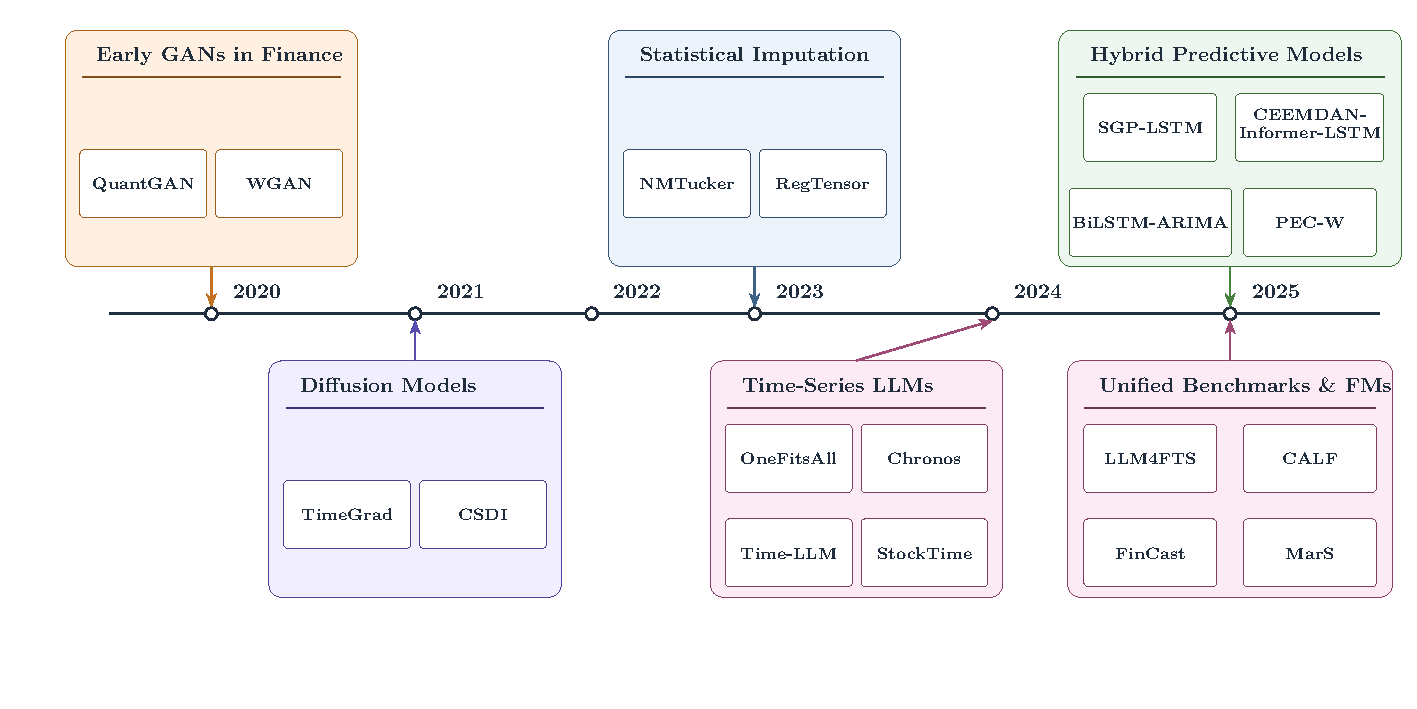
\includegraphics[width=0.98\linewidth]{separate_figures/Figure1.pdf}
\caption{\textbf{Evolution of Financial Time-Series Generation techniques over the past decade.} Timeline of representative milestones in financial time-series generation (FTSG) from 2020 to early 2026. Colored cards along the central axis denote technical families: coral pink for adversarial generative architectures (GANs), steel blue for diffusion and score-based models, amber orange for time-series foundation models and adapted large language models (LLMs), and sage green for classical statistical, tensor factorization, and deep predictive baselines. Key models include NMTucker (Non-negative Matrix Tucker factorization), RegTensor, NDDP (Nonlinear Diffusion Drift Process), PEC-W, SGP-LSTM, TimeGrad, CSDI, Time-LLM, StockTime, CALF (Cross-modal Aligned Foundation model), FinCast, and MarS (Multi-Agent Market Simulator). White circular markers denote calendar years 2020, 2021, 2023, 2024, and 2025; directed arrows align each contribution to its release year.}
\label{fig:timeline}
\end{figure}

\newpage

\begin{figure}[!ht]
\centering
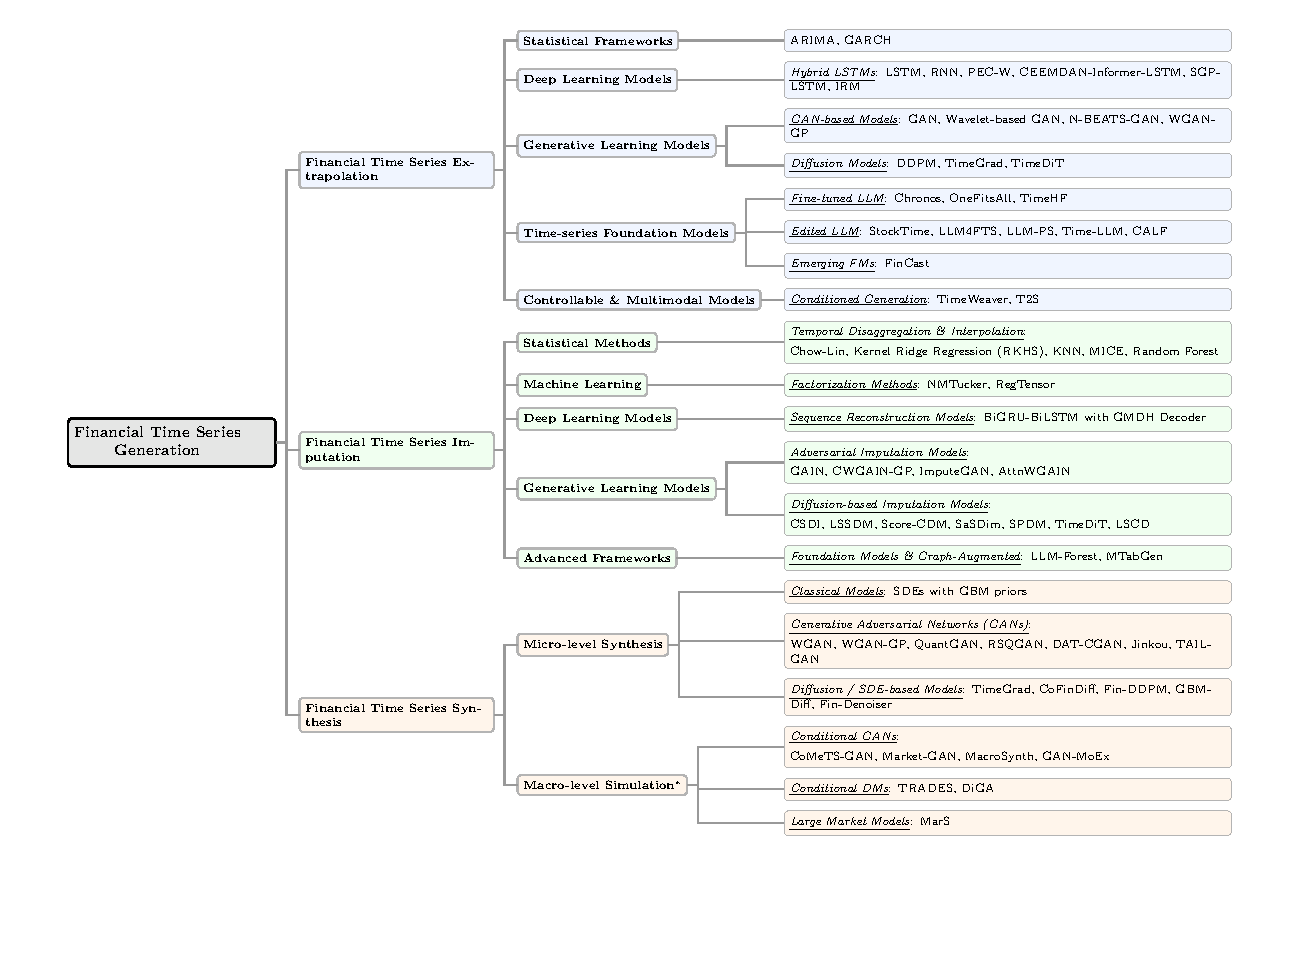
\includegraphics[width=0.98\linewidth]{separate_figures/Figure2.pdf}
\caption{\textbf{Hierarchical two-level taxonomy of financial time-series generation.} Systematic classification structure decoupling financial generation tasks from generative modeling paradigms. The primary tree root partitions FTSG into three functional task branches. Light blue shaded blocks designate the forward-looking Financial Time-Series Extrapolation (FTSE) branch, spanning statistical autoregressive models, deep sequential networks, adversarial frameworks, diffusion dynamics, and foundation model adaptations. Light green shaded blocks designate the bidirectional Financial Time-Series Imputation (FTSI) branch, covering temporal disaggregation, tensor factorization baselines, recurrent encoders, generative adversarial imputers, score-based diffusion methods, and graph-augmented transformer architectures. Light orange shaded blocks designate the generative Financial Time-Series Synthesis (FTSS) branch, categorized into micro-level asset return synthesis and macro-level market microstructure simulation across conditional GANs, diffusion models, and large market agent simulators. Grey orthogonal branch lines indicate conceptual inheritance. The asterisk ($^*$) indicates that only purely generative model families are enumerated in the synthesis branch.}
\label{fig:taxonomy}
\end{figure}

\newpage

\begin{figure}[!ht]
\centering
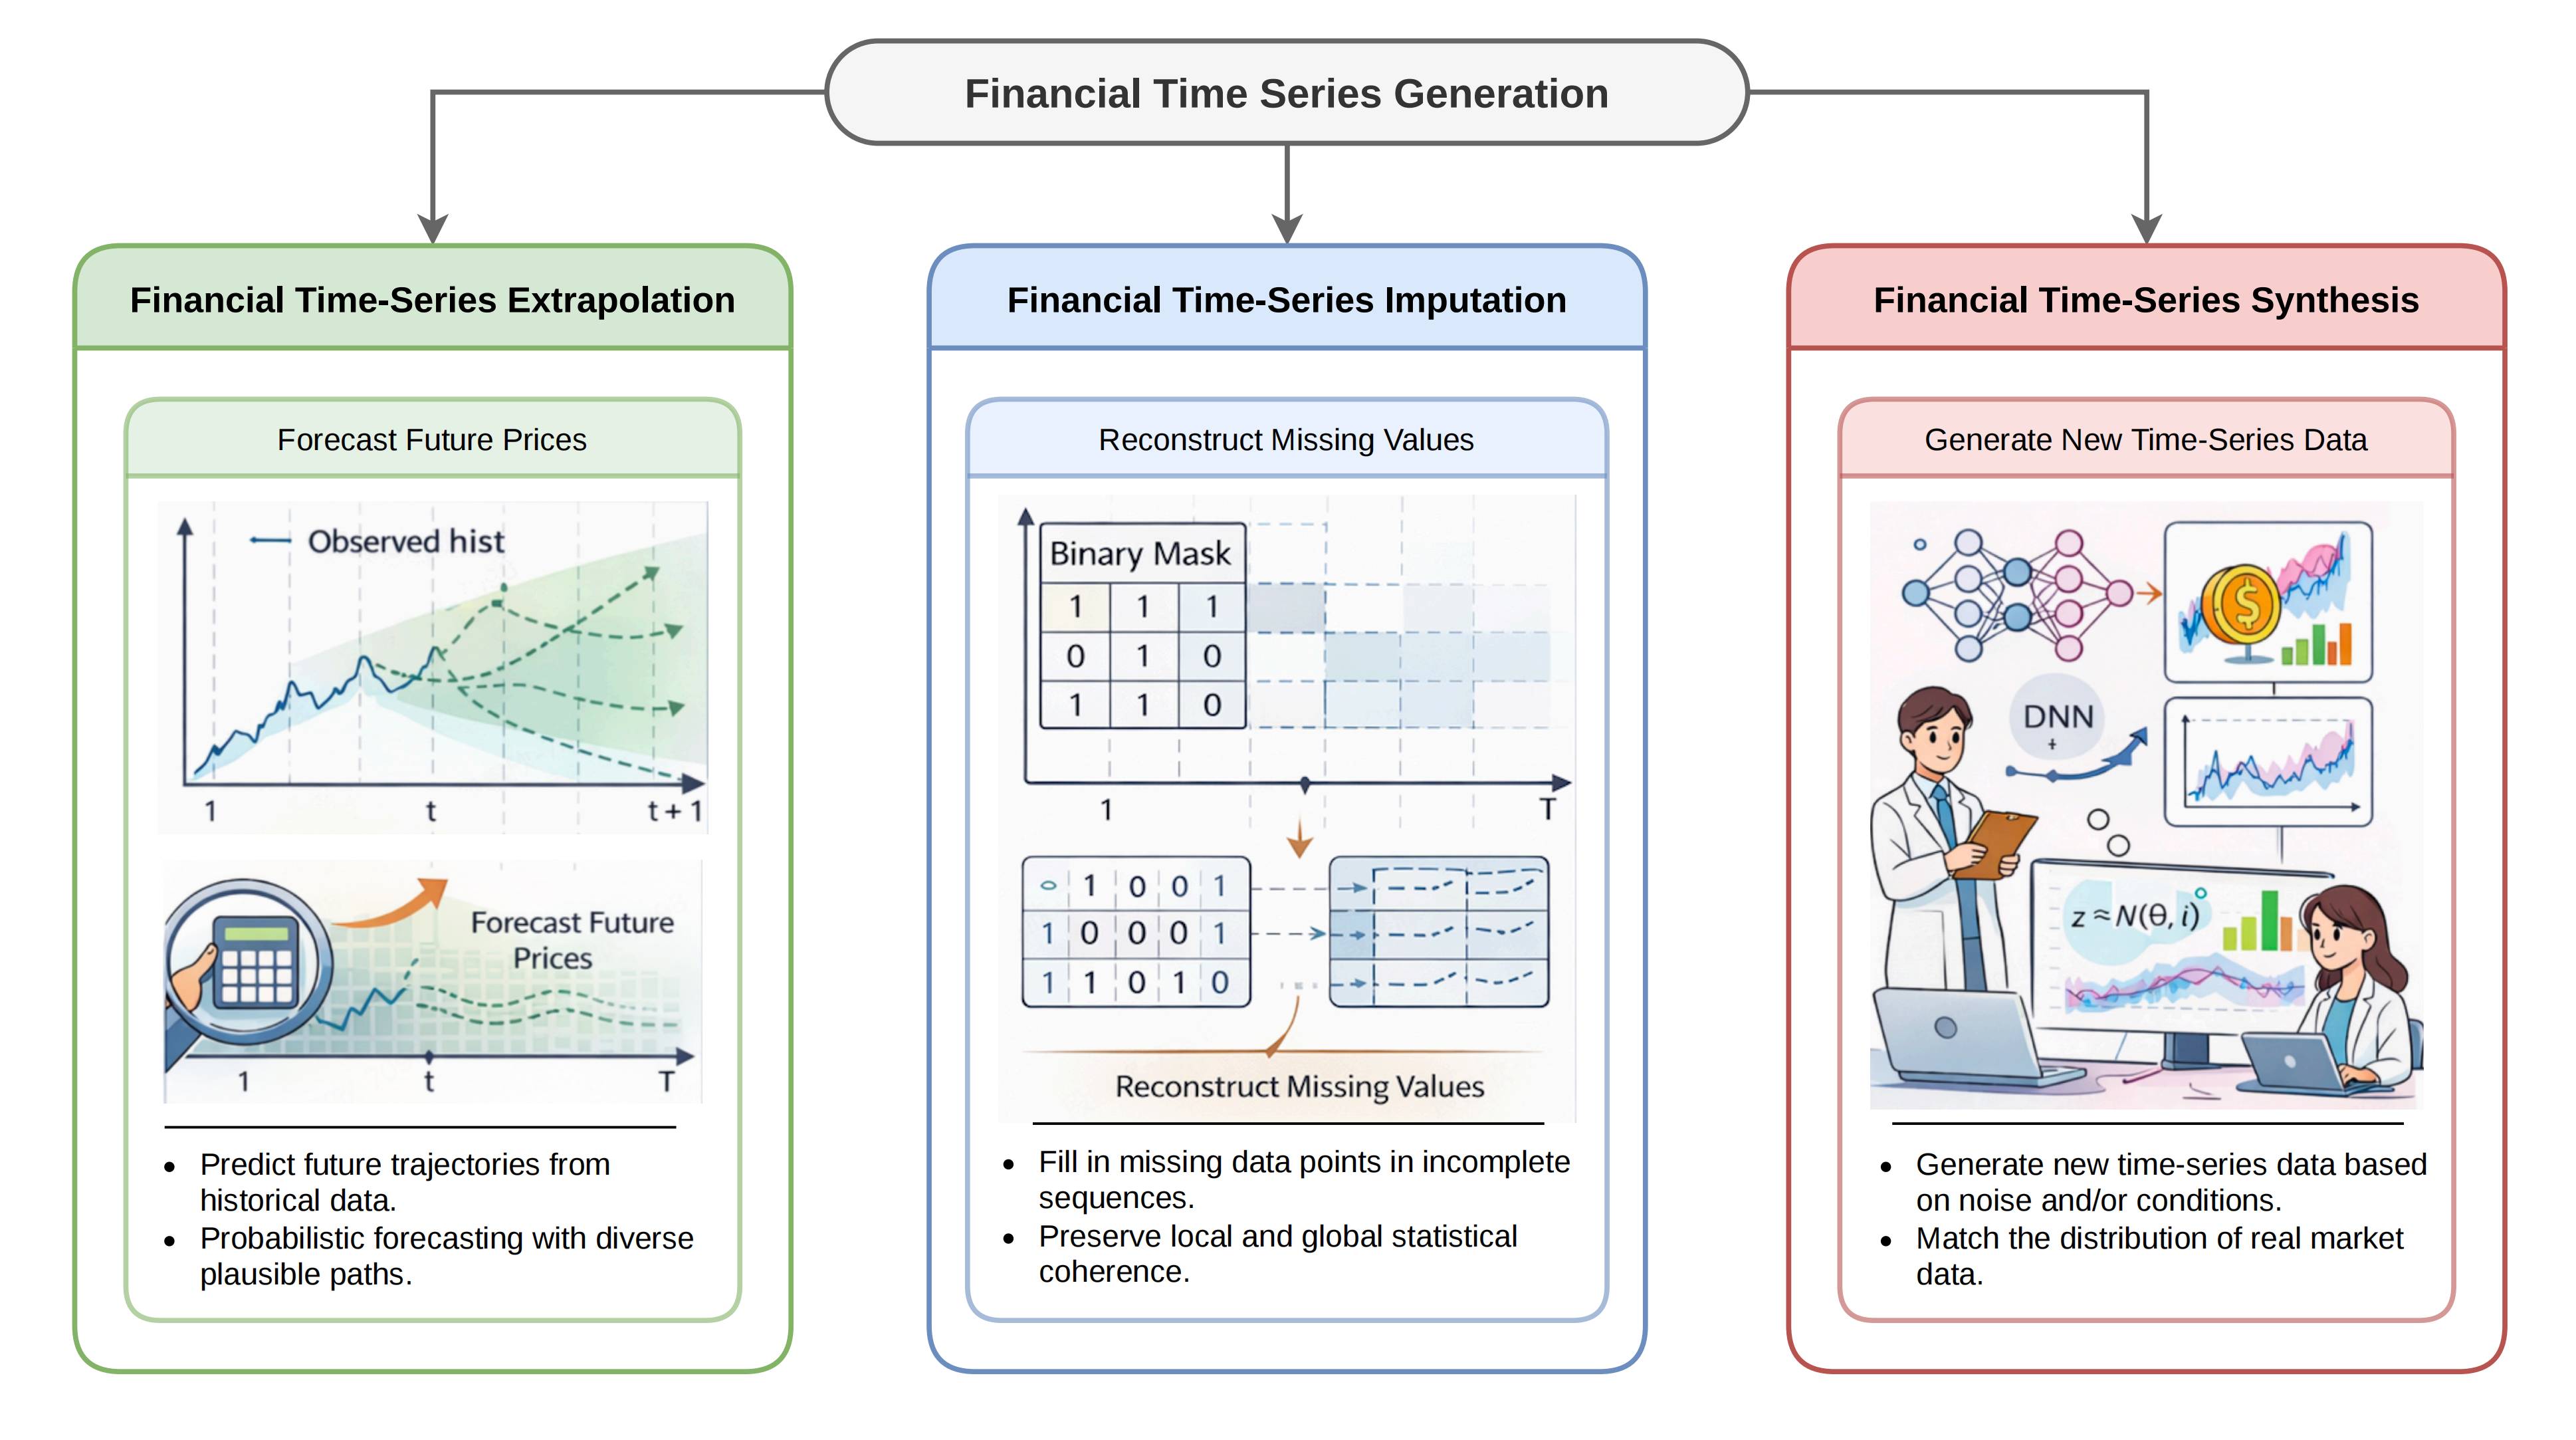
\includegraphics[width=0.9\linewidth]{final_figures/comparison_00.png}
\caption{\textbf{Structural comparison of core financial time-series generation tasks.} Schematic representation contrasting the conditioning context, temporal boundary conditions, and output targets across three generation formulations. \textbf{a,} Financial time-series extrapolation (FTSE): conditional forward-looking trajectory continuation, where a past historical prefix (solid line markers) guides probabilistic generation of unobserved future steps (dashed continuation markers). \textbf{b,} Financial time-series imputation (FTSI): closed-format bidirectional reconstruction, where known observed points bound an interval of missing or corrupted values, reconstructed via temporal and cross-sectional conditioning. \textbf{c,} Synthetic sequence generation (FTSS): unconditional or attribute-guided manifold creation from latent Gaussian noise and market condition vectors, simulating realistic synthetic price paths and order books without pointwise historical alignment.}
\label{fig:tasks}
\end{figure}

\newpage

\begin{figure}[!ht]
\centering
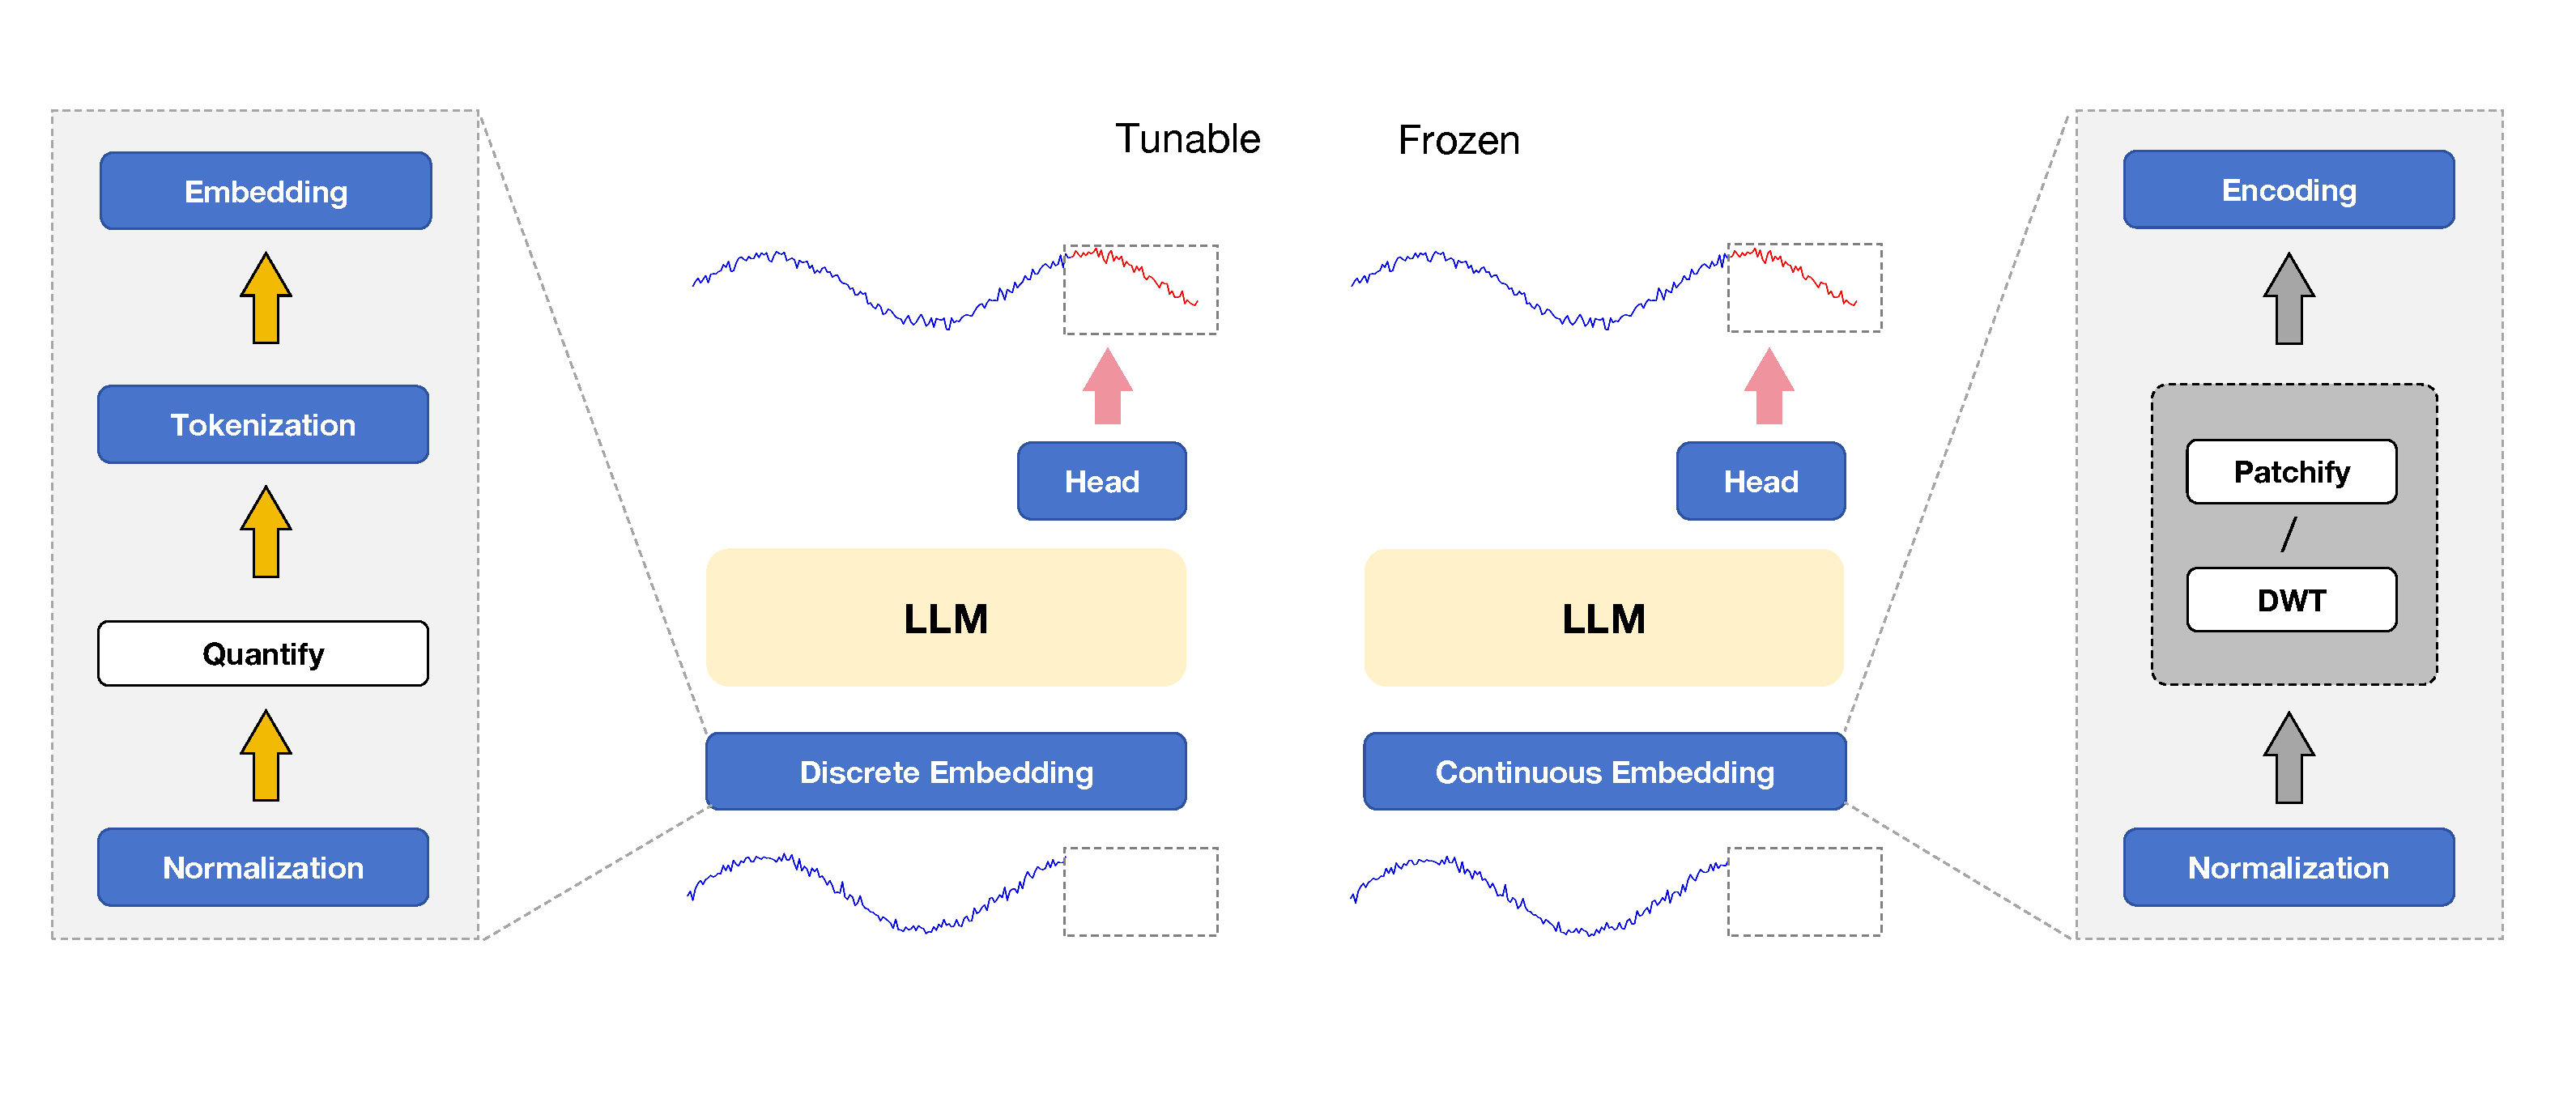
\includegraphics[width=0.8\textwidth,keepaspectratio]{final_figures/DiffWithDiscreteContinous.pdf}
\caption{\textbf{Architectural paradigms for adapting foundation models to financial time series.} Schematic diagram contrasting tokenization- and patch-based fine-tuning against model editing and prompt reprogramming. \textbf{a,} Fine-tuning paradigm (left): numerical continuous time series are transformed into discrete token vocabularies via quantile binning or linear patch projection layers, followed by backpropagation through transformer backbones. \textbf{b,} Prompt reprogramming and cross-modal model editing paradigm (right): a frozen foundation model backbone receives auxiliary steering signals from textual market prompts, cross-attention alignment bridges, and lightweight adapter modules, avoiding full-parameter gradient updates while preserving numerical precision. Blue rectangular boxes represent time-series input vectors, purple layered blocks denote multi-head self-attention transformer layers, and green highlighted modules represent learnable cross-modal projection heads.}
\label{fig:llm_comparison}
\end{figure}

\newpage

\begin{figure}[!ht]
\centering
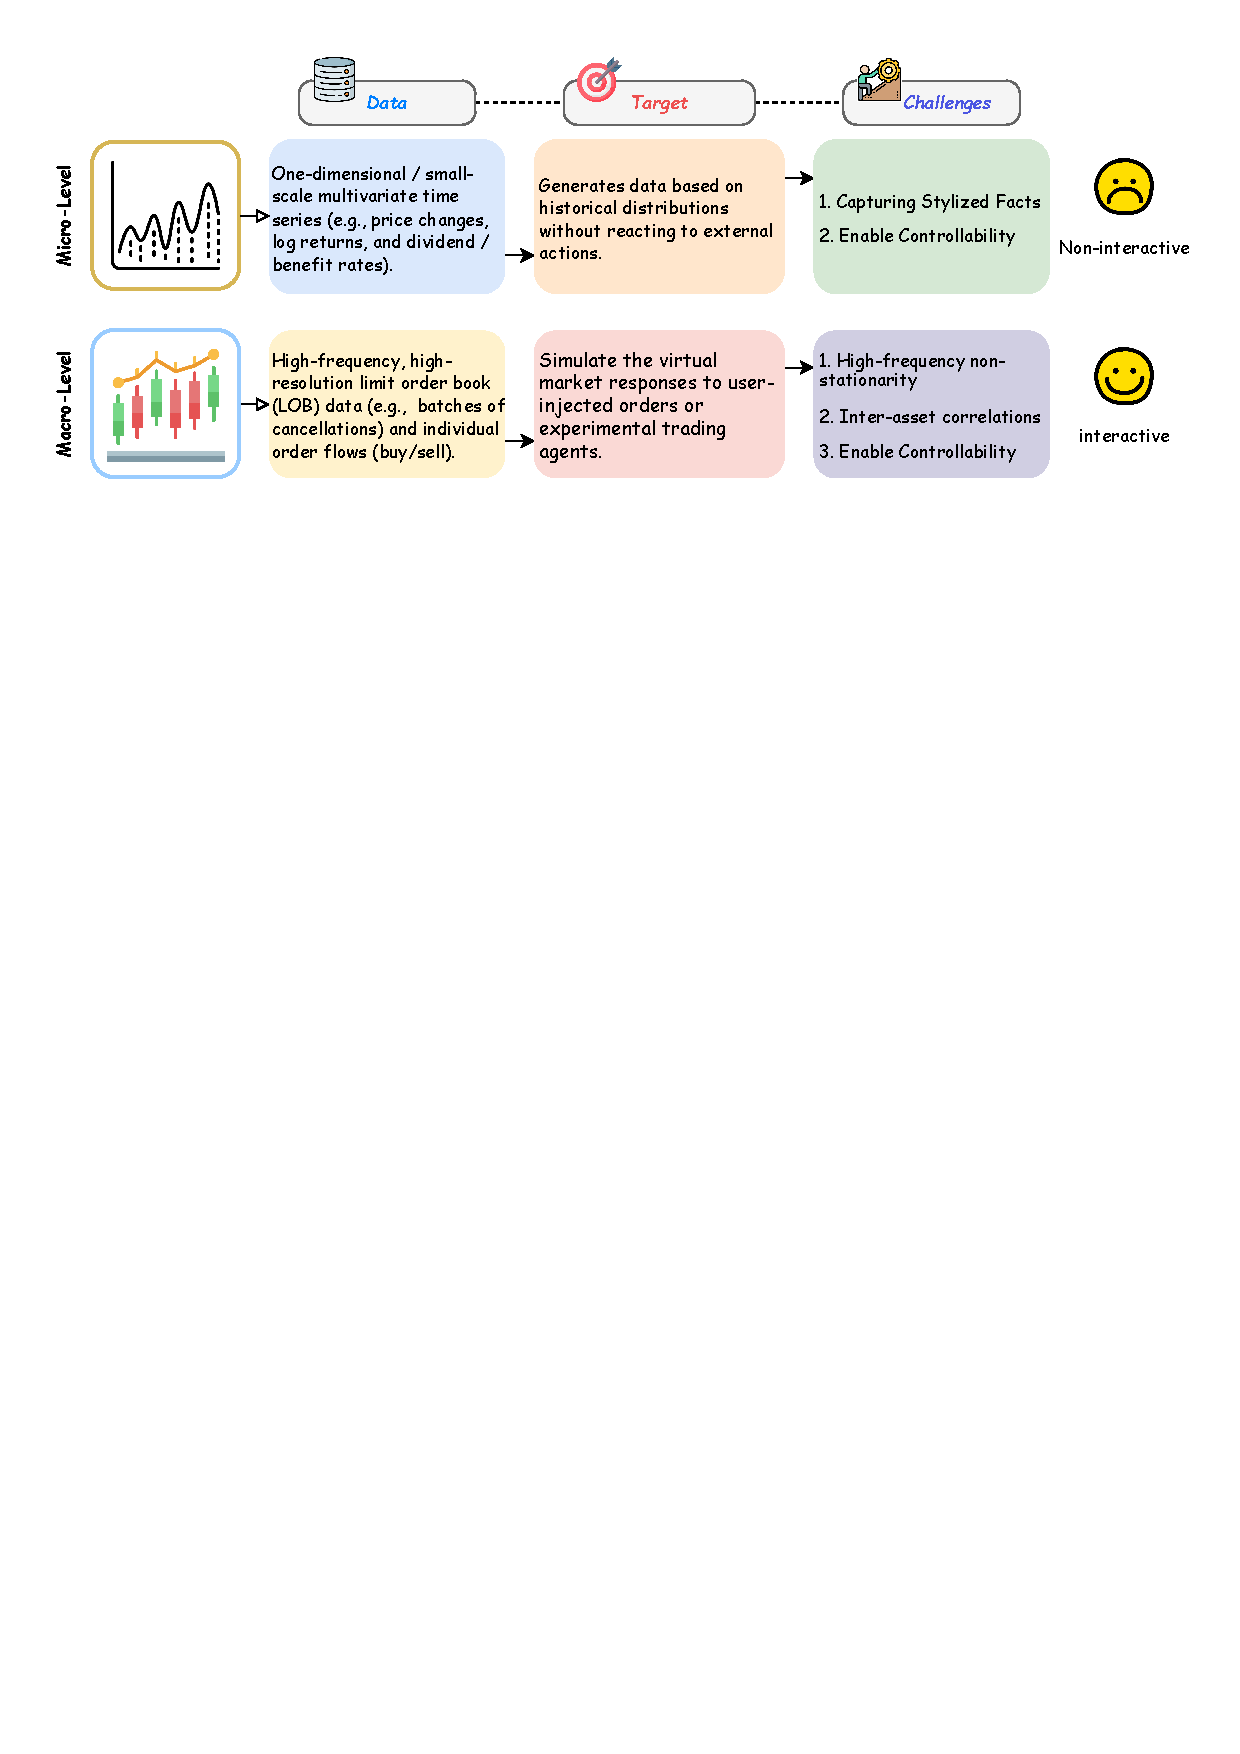
\includegraphics[width=0.8\textwidth,keepaspectratio]{final_figures/FTSA.pdf}
\caption{\textbf{Multi-scale architectural paradigms for financial time-series synthesis.} Conceptual comparison of synthetic sequence generation partitioned into micro-level return modeling and macro-level market simulation. \textbf{a,} Micro-level synthesis (left): univariate or low-dimensional asset return path generation via Wasserstein GANs with temporal convolutional backbones and score-matching diffusion models, engineered to preserve stylized econometric facts such as heavy tails, absence of linear autocorrelation, and volatility clustering. \textbf{b,} Macro-level market simulation (right): multi-agent and limit order book (LOB) queue modeling where generative architectures simulate asynchronous order message flows, bid-ask depth ladders, cross-asset spillover correlations, and macroeconomic counterfactual shock scenarios under regulatory and privacy constraints. Color shading highlights the transition from low-dimensional statistical moments to high-dimensional interactive market topologies.}
\label{fig:ftss_comparison}
\end{figure}

\newpage

\begin{figure}[!ht]
\centering
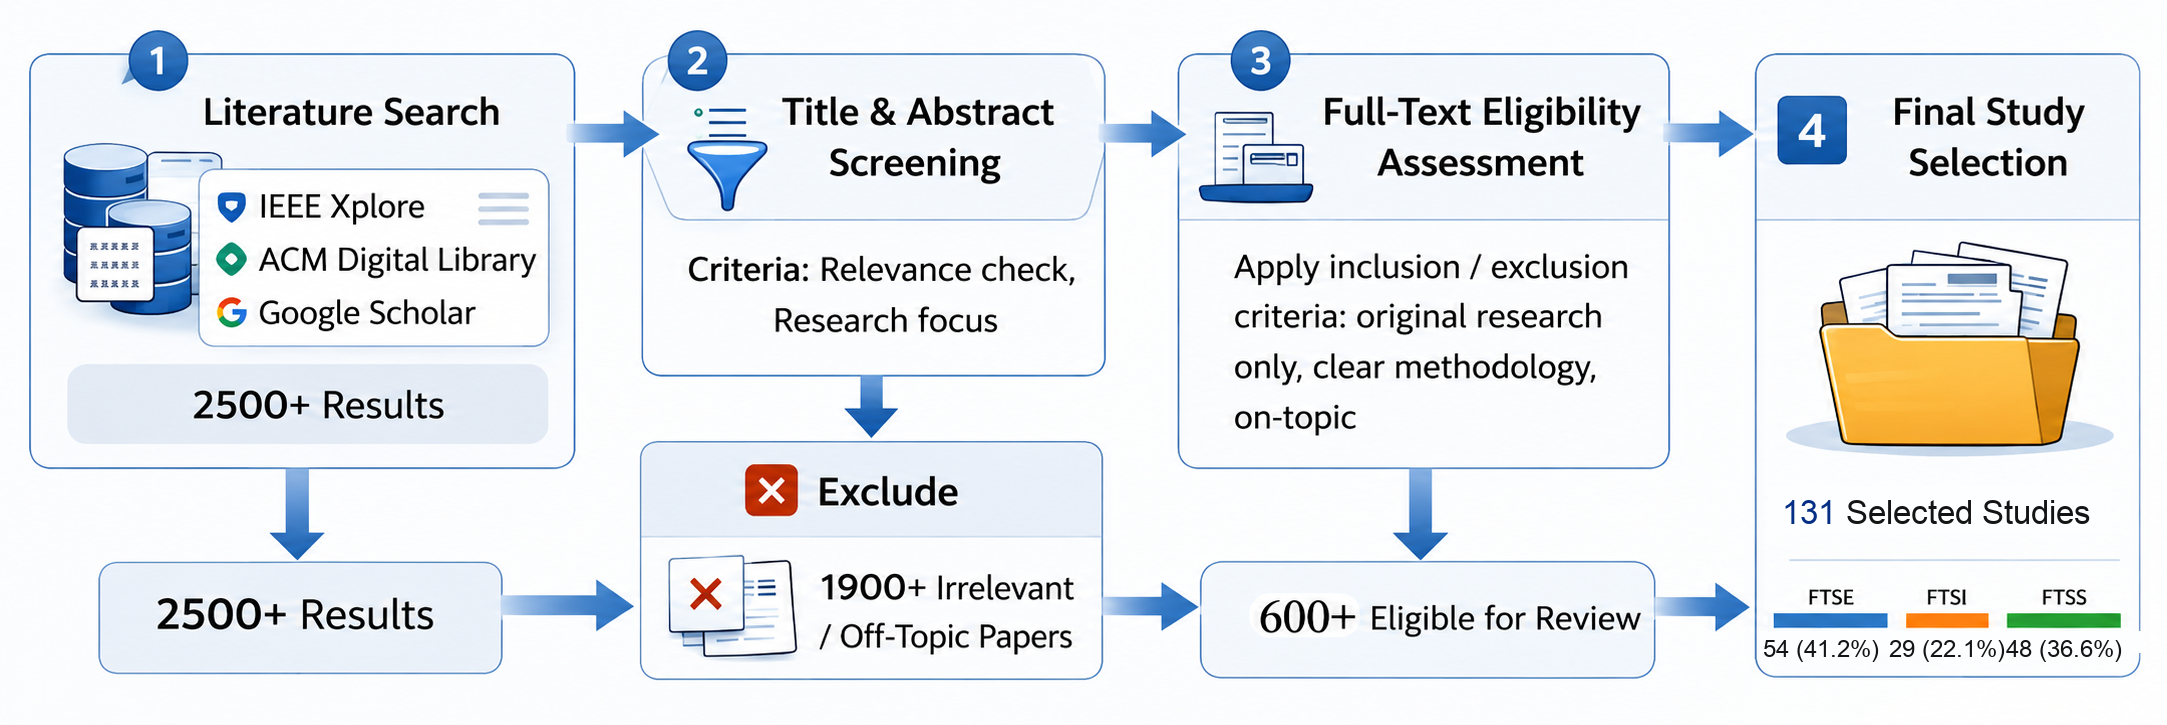
\includegraphics[width=0.95\textwidth,keepaspectratio]{final_figures/filter_pipeline.png}
\caption{\textbf{Literature identification and PRISMA screening pipeline.} Flow diagram illustrating the systematic retrieval, multi-stage screening, and eligibility determination process compliant with the PRISMA 2020 framework. Blue rectangular boxes represent initial literature identification across primary databases (Google Scholar, DBLP, Web of Science, Scopus, arXiv) and duplicate removal. Orange rectangular boxes denote title and abstract screening stages with corresponding exclusion criteria. Red dashed borders and rightward branching callouts indicate excluded records at each phase along with explicit rationales (non-financial domains, deterministic point forecasting without generative distributions, non-reproducible records). Green solid rectangular boxes indicate the final corpus of 130 retained studies meeting all eligibility criteria, partitioned into three task categories: financial time-series extrapolation, imputation, and data synthesis. Detailed quantitative counts for each filtering phase are recorded in the accompanying retrieval statistics table.}
\label{fig:lit_dist}
\end{figure}


\newpage
\section*{Tables}

\begin{table*}[!ht]
\centering
\scriptsize
\caption{Comparison of this survey with the six prior surveys cited in the literature comparison. \textbf{FTSE/FTSI/FTSS} columns use \checkmark/\texttimes\ for whether the sub-task is a first-class topic ($\triangle$ = mentioned but no dedicated section). \textbf{Eval.} distinguishes a unified \emph{protocol} from per-paper \emph{metrics}. \textbf{Datasets} indicates whether financial benchmarks are inventoried. \textbf{\# refs} is the count of references cited in each survey. \textbf{Window} is the publication-year range of each survey's references.}
\label{tab:related_surveys}
\renewcommand{\arraystretch}{1.18}
\begin{tabular}{l c c c l l c l}
\toprule
\textbf{Survey} & \textbf{FTSE} & \textbf{FTSI} & \textbf{FTSS} & \textbf{Eval.} & \textbf{Datasets} & \textbf{\# refs} & \textbf{Window} \\
\midrule
\citet{Survey1}            & \checkmark & \texttimes & \texttimes & None    & Multimodal TS & 93  & 2005--2024 \\
\citet{Survey2}            & \checkmark & $\triangle$ & \texttimes & None    & General TS        & 123 & 2017--2024 \\
\citet{Survey3}            & \checkmark & \texttimes & \texttimes & Metrics & General TS    & 287 & 2000--2024 \\
\citet{Survey4}            & \checkmark & \texttimes & \texttimes & Metrics & General TS    & 285 & 2000--2024 \\
\citet{FinSurvey1}         & \checkmark & \texttimes & \texttimes & Metrics & Financial NLP     & 318 & 2001--2024 \\
\citet{FinSurvey3}         & \checkmark & \texttimes & \texttimes & Metrics & Financial TS      & 115 & 2018--2023 \\
\midrule
\textbf{This survey}      & \checkmark & \checkmark & \checkmark & \textbf{Protocol} & \textbf{Financial TS} & \textbf{130} & \textbf{2021--early 2026} \\
\bottomrule
\end{tabular}
\end{table*}

\vspace{2em}

\begin{table*}[!ht]
\centering
\scriptsize
\caption{Unified Task-Technique-Evaluation Mapping for Financial Time-Series Generation.}
\label{tab:mapping}
\resizebox{\textwidth}{!}{
\begin{tabular}{p{2cm} p{2.5cm} p{5.5cm} p{2.5cm} p{3.5cm}}
\toprule
\textbf{Task} & \textbf{Model Family} & \textbf{Representative Approaches} & \textbf{Data Type} & \textbf{Primary Evaluation} \\
\midrule
\multirow{3}{*}{\textbf{Extrapolation}} & Deep Sequence & SGP-LSTM \citep{SGP-LSTM1} & Prices, Returns & MSE, Directional Accuracy \\
 & Diffusion Models & TimeGrad \citep{rasul2021timegrad} & Multivariate Series & CRPS, Predictive Likelihood \\
 & Foundation Models & Chronos \citep{ansari2024chronos}, FinCast \citep{zhu2025fincast} & Multi-asset & Zero-shot MSE, MAE \\
\midrule
\multirow{2}{*}{\textbf{Imputation}} & Tensor Methods & RegTensor \citep{zhou2023regtensor} & Fundamentals & Reconstruction Error \\
 & Diffusion Models & CSDI \citep{tashiro2021csdi}, TimeDiT \citep{TimeDiT} & Missing Prices & Temporal Coherence \\
\midrule
\multirow{3}{*}{\textbf{Synthesis}} & GANs & QuantGAN \citep{wiese2020} & Returns & Stylized Facts \\
 & Diffusion Models & CoFinDiff \citep{tanaka2025cofindiff} & Scenarios & Distributional Fidelity \\
 & Controllable & Market-GAN \citep{xia2024market} & Order Flow (LOB) & Downstream Utility \\
\bottomrule
\end{tabular}
}
\end{table*}

\vspace{2em}

\begin{table*}[!ht]
\centering
\scriptsize
\caption{Comprehensive Comparison of Financial Time-Series Extrapolation Paradigms}
\label{tab:extrapolation_comparison}
\renewcommand{\arraystretch}{1.3}
\resizebox{\textwidth}{!}{
\begin{tabular}{lp{3.5cm}p{4cm}p{4.5cm}p{4cm}}
\toprule
\textbf{Paradigm} & \textbf{Output Format} & \textbf{Key Strengths} & \textbf{Primary Limitations} & \textbf{Typical Financial Use Cases} \\
\midrule
\textbf{Predictive Models} & Deterministic point forecasts & Extremely fast inference; highly interpretable methodologies. & Lacks robust uncertainty quantification; fails to model tail risks. & High-frequency trading; algorithmic order execution. \\
\textbf{GANs} & Sampled stochastic trajectories & Produces sharp, multi-modal sequences without iterative sampling. & Prone to severe training instability and mode collapse. & Scenario generation; counterfactual stress testing. \\
\textbf{Diffusion Models} & Sampled stochastic trajectories & Achieves strong distributional fidelity and stable convergence. & Iterative sampling process induces prohibitive computational latency. & Risk management; complex portfolio optimization. \\
\textbf{Foundation Models} & Zero-shot probabilistic forecasts & Exhibits promising cross-domain generalization and rapid adaptability. & Suffers from potential hallucination and difficult text-series data alignment. & Dynamic asset allocation; broad market backtesting. \\
\bottomrule
\end{tabular}
}
\end{table*}

\newpage

\begin{table*}[!ht]
\centering
\scriptsize
\caption{Comparative Analysis of Financial Time-Series Imputation Frameworks}
\label{tab:imputation_comparison}
\renewcommand{\arraystretch}{1.3}
\resizebox{\textwidth}{!}{
\begin{tabular}{lp{3.5cm}p{4cm}p{4.5cm}}
\toprule
\textbf{Methodology} & \textbf{Core Mechanism} & \textbf{Key Advantages} & \textbf{Primary Limitations} \\
\midrule
\textbf{Matrix/Tensor Completion} & Low-rank factorization & Highly computationally efficient; effective on sparse data. & Fails to capture non-linear volatility clustering. \\
\textbf{Tree-Based (Random Forest)} & Non-linear ensemble regression & Extremely robust to high missing rates (e.g., 50\%+). & Struggles with high-frequency temporal dependencies. \\
\textbf{GAN-Based Models} & Adversarial distribution matching & Sharp interpolations; mitigates drift via gradient penalties. & Mode collapse; unstable training on extreme outages. \\
\textbf{Diffusion Models} & Conditional reverse denoising & State-of-the-art fidelity; preserves cross-asset correlations. & High inference latency prohibitive for real-time systems. \\
\textbf{LLM/Graph Frameworks} & Bipartite graphs \& textual prompting & Excels on mixed-type (categorical/numerical) tabular data. & Heavy computational footprint; context-window limits. \\
\bottomrule
\end{tabular}
}
\end{table*}

\vspace{2em}

\begin{table*}[!ht]
\centering
\scriptsize
\caption{Comparative Overview of Financial Time-Series Synthesis Paradigms}
\label{tab:synthesis_comparison}
\renewcommand{\arraystretch}{1.3}
\resizebox{\textwidth}{!}{
\begin{tabular}{lp{3.5cm}p{4cm}p{4.5cm}}
\toprule
\textbf{Model Paradigm} & \textbf{Core Methodology} & \textbf{Primary Strengths} & \textbf{Key Limitations} \\
\midrule
\textbf{Wasserstein GANs} & Adversarial minimax game with Earth Mover's distance & Rapid inference; highly effective for targeted metric alignment. & Susceptible to mode collapse; struggles with microstructural nuance. \\
\textbf{Diffusion \& SDEs} & Iterative forward noising and reverse score-matching & Exceptional distributional fidelity; easily integrates financial priors (e.g., GBM). & Computationally intensive sampling process limits real-time utility. \\
\textbf{Large Market Models} & Transformer-based discrete sequence modeling & Scales to asynchronous tick data; enables interactive agent simulation. & Requires massive computational infrastructure and vast order-flow datasets. \\
\textbf{DP-Generators} & Differentially private gradient clipping & Ensures strict regulatory compliance and data anonymization. & Incurs a harsh trade-off between privacy bounds ($\epsilon$) and data utility. \\
\bottomrule
\end{tabular}
}
\end{table*}

\vspace{2em}

\begin{table*}[!ht]
\centering
\scriptsize
\caption{A Unified Evaluation Checklist for Financial Time-Series Generation.}
\label{tab:evaluation_checklist}
\resizebox{\textwidth}{!}{
\begin{tabular}{p{3.5cm} p{5.5cm} p{3.5cm} p{4cm}}
\toprule
\textbf{Evaluation Dimension} & \textbf{Key Metrics / Methods} & \textbf{Primary Task Suitability} & \textbf{Reflects Financial Validity?} \\
\midrule
\textbf{Point-wise Accuracy} & MSE, MAE, RMSE, MAPE & Extrapolation, Imputation & Low (Ignores market dynamics) \\
\textbf{Distributional Fidelity} & Wasserstein Distance, MMD, KL Divergence, Cross-Correlation & Synthesis, Extrapolation & Medium (Captures static shapes) \\
\textbf{Stylized Facts} & ACF of squared returns, Tail Index, Kurtosis, Leverage effect tests & Synthesis, Simulation & High (Domain-specific realism) \\
\textbf{Downstream Utility} & Train-on-Synthetic, Test-on-Real (TSTR); Train-on-Real, Test-on-Real (TRTR); Sharpe Ratio of trained agents; VaR/ES accuracy & All Tasks & High (Practical applicability) \\
\textbf{Privacy \& Security} & Distance-to-Closest Record (DCR), Differential Privacy $\epsilon$ & Synthesis (Data Sharing) & N/A (Focuses on compliance) \\
\bottomrule
\end{tabular}
}
\end{table*}

\newpage

\begin{table*}[!ht]
\centering
\scriptsize
\caption{Summary of Recent Financial Time-Series Generation Benchmarks.}
\label{tab:datasets}
\begin{tabular}{p{3.5cm} c p{4.5cm} c c}
\toprule
\textbf{Dataset / Benchmark} & \textbf{Tasks} & \textbf{Primary Data Sources} & \textbf{Split Ratio} & \textbf{Scale (Approx.)} \\
\midrule
\textbf{FinTSB} \citep{hu2025fintsb} & Extrapolation / Imputation & Chinese A-share, NYSE, NASDAQ & 7:1:2 & 150M points \\
\rowcolor{gray!10}
\textbf{GIFT-EVAL} \citep{GIFT-EVAL} & Forecasting & 27 datasets (Stock, Crypto, FX, etc.) & Various & 144,380 series \\
\textbf{TFB} \citep{TFB} & Forecasting & Broad finance domain & Various & 2.1M series \\
\rowcolor{gray!10}
\textbf{FinTSBridge} \citep{wang2025fintsbridge} & Extrapolation / Imputation & S\&P 500, NASDAQ, FTSE, CSI 300 & 7:1:2 & 86,978 series \\
\textbf{TSGBench} \citep{ang2023tsgbench} & Synthesis / Simulation & GOOGL, Global Exchanges & 9:0:1 & 13,213 series \\
\textbf{CTBench} \citep{ang2025ctbench} & Synthesis & Cryptocurrencies on Binance & 9:0:1 & 530 series \\
\textbf{FinMultiTime} \citep{FinMultiTime} & Extrapolation & S\&P 500, HS 300 & N/A & 6M points \\
\bottomrule
\end{tabular}
\end{table*}

\vspace{2em}

\begin{table*}[!ht]
\centering
\scriptsize
\caption{Literature Retrieval and Screening Statistics.}
\label{tab:retrieval_stats}
\begin{tabular}{p{5cm} p{2cm} p{2cm} p{3cm}}
\toprule
\textbf{Screening Stage} & \textbf{Count} & \textbf{Retained} & \textbf{Primary Reason for Exclusion} \\
\midrule
Initial Keyword Search & 2,568 & 2,568 & N/A \\
Title/Abstract Screening & 2,568 & 604 & Not financial data / Pure deterministic forecasting \\
Full-text Review & 604 & \textbf{130} & Weak financial validation / Duplicated preprints \\
\midrule
\multicolumn{4}{l}{\textbf{Primary Task Assignment}} \\
\quad Extrapolation & & 54 & \\
\quad Imputation & & 29 & \\
\quad Synthesis / Simulation & & 47 & \\
\bottomrule
\end{tabular}
\begin{flushleft}
\textit{Note: Each of the 130 retained studies is assigned to exactly one primary task category; cross-cutting contributions (e.g., forecasting with imputation or synthesis with scenario conditioning) are discussed in the relevant sections but are not double-counted.}
\end{flushleft}
\end{table*}


\end{document}
